% Please make sure you insert your
% data according to the instructions in PoSauthmanual.pdf
\documentclass{PoS}

\title{Rare decays at CMS}

\ShortTitle{Rare decays at CMS}

\author{\speaker{J\'onatan Piedra}\thanks{On behalf of the CMS Collaboration.}\\
        IFCA (CSIC - Universidad de Cantabria)\\
        E-mail: \email{piedra@cern.ch}}

%\author{Another Author\\
%        Affiliation\\
%        E-mail: \email{...}}

\abstract{Searches for flavour changing neutral currents (FCNC) in events with
top quarks and the Z or the Higgs boson are presented by the CMS Collaboration.
These searches use proton-proton collision events taken by the CMS experiment
at the Large Hadron Collider (LHC), built by the European Organization for
Nuclear Research (CERN). Upper limits at 95\% confidence level are set on the
branching fractions of ${\rm t \to qZ}$ and ${\rm t \to qH}$ decays. In addition,
angular distributions of ${\rm B^0}$ and ${\rm B^+}$ decays are presented. These
measurements are found to be consistent with predictions based on the standard
model.}

\FullConference{XIV International Conference on Heavy Quarks and Leptons (HQL2018)\\
		May 27 - June 1, 2018\\
		Yamagata Terrsa, Yamagata, Japan}


\begin{document}


%-------------------------------------------------------------------------------
\section{FCNC in ${\rm tZq \to 3\ell}$}
%-------------------------------------------------------------------------------

In the standard model (SM), FCNC are
forbidden at tree level and highly suppressed at higher orders. Several
extensions of the SM enhance the FCNC branching fractions and can be probed at
the LHC; the new couplings can also provide for flavour changing single top
quark production in association with a Z or a Higgs boson.
This analysis~\cite{top-17-017} uses proton-proton collision data accumulated
during the 2016 running period, corresponding to an integrated luminosity of
${\rm 35.9~fb^{-1}}$ at a centre-of-mass energy of 13~TeV collected by the CMS
detector~\cite{cms-detector}. The analysis focuses on the experimental search
for evidence of FCNC
vertex (referred to as tZq) with a top quark, a Z boson, and a quark q that is
either up or charm. In the final state we expect one jet originating from a b quark,
a W boson, a Z boson, and (in the case of FCNC top quark decay) a jet originating
from the up or charm quark. As we limit the analysis to electronic and muonic
decays of both the
W and the Z boson, events are selected requiring exactly 3 leptons containing one
opposite sign, same flavour pair; at least 1 jet and at most 3 jets; and the
transverse mass of the W boson below 300~GeV. Four different lepton channels are
considered (3e, 2e1$\mu$, 1e2$\mu$, 3$\mu$) and two signal regions are constructed
using the jet multiplicity, the single top quark (STSR) and the top quark pair
(TTSR) FCNC. A simultaneous global fit is performed taking into account
both signal regions and background regions for the four lepton channels with the
help of boosted decision trees (BDT) used to discriminate between signal and
background. The resulting discriminating output variables from each BDT are
shown in Figure~\ref{fig:TOP-17-017_Figure_003}. The signal strength and significance
are computed treating all systematic uncertainties as nuisance parameters and are
constrained from the fit which uses templates in the different signal and
background regions for each of the four different lepton channels. The resulting
observed (expected) limits where both couplings are non-vanishing are shown in
Figure~\ref{fig:TOP-17-017_Figure_007}. No significant deviation is observed from
the predicted background. Observed (expected) upper limits at 95\% CL are set on
the branching fractions of top quark decays:
${\cal B}({\rm t \to uZ}) < 0.024\%~(0.015\%)$ and
${\cal B}({\rm t \to cZ}) < 0.045\%~(0.037\%)$, assuming one non-vanishing
coupling at a time.


\begin{figure}[htb]
\centering
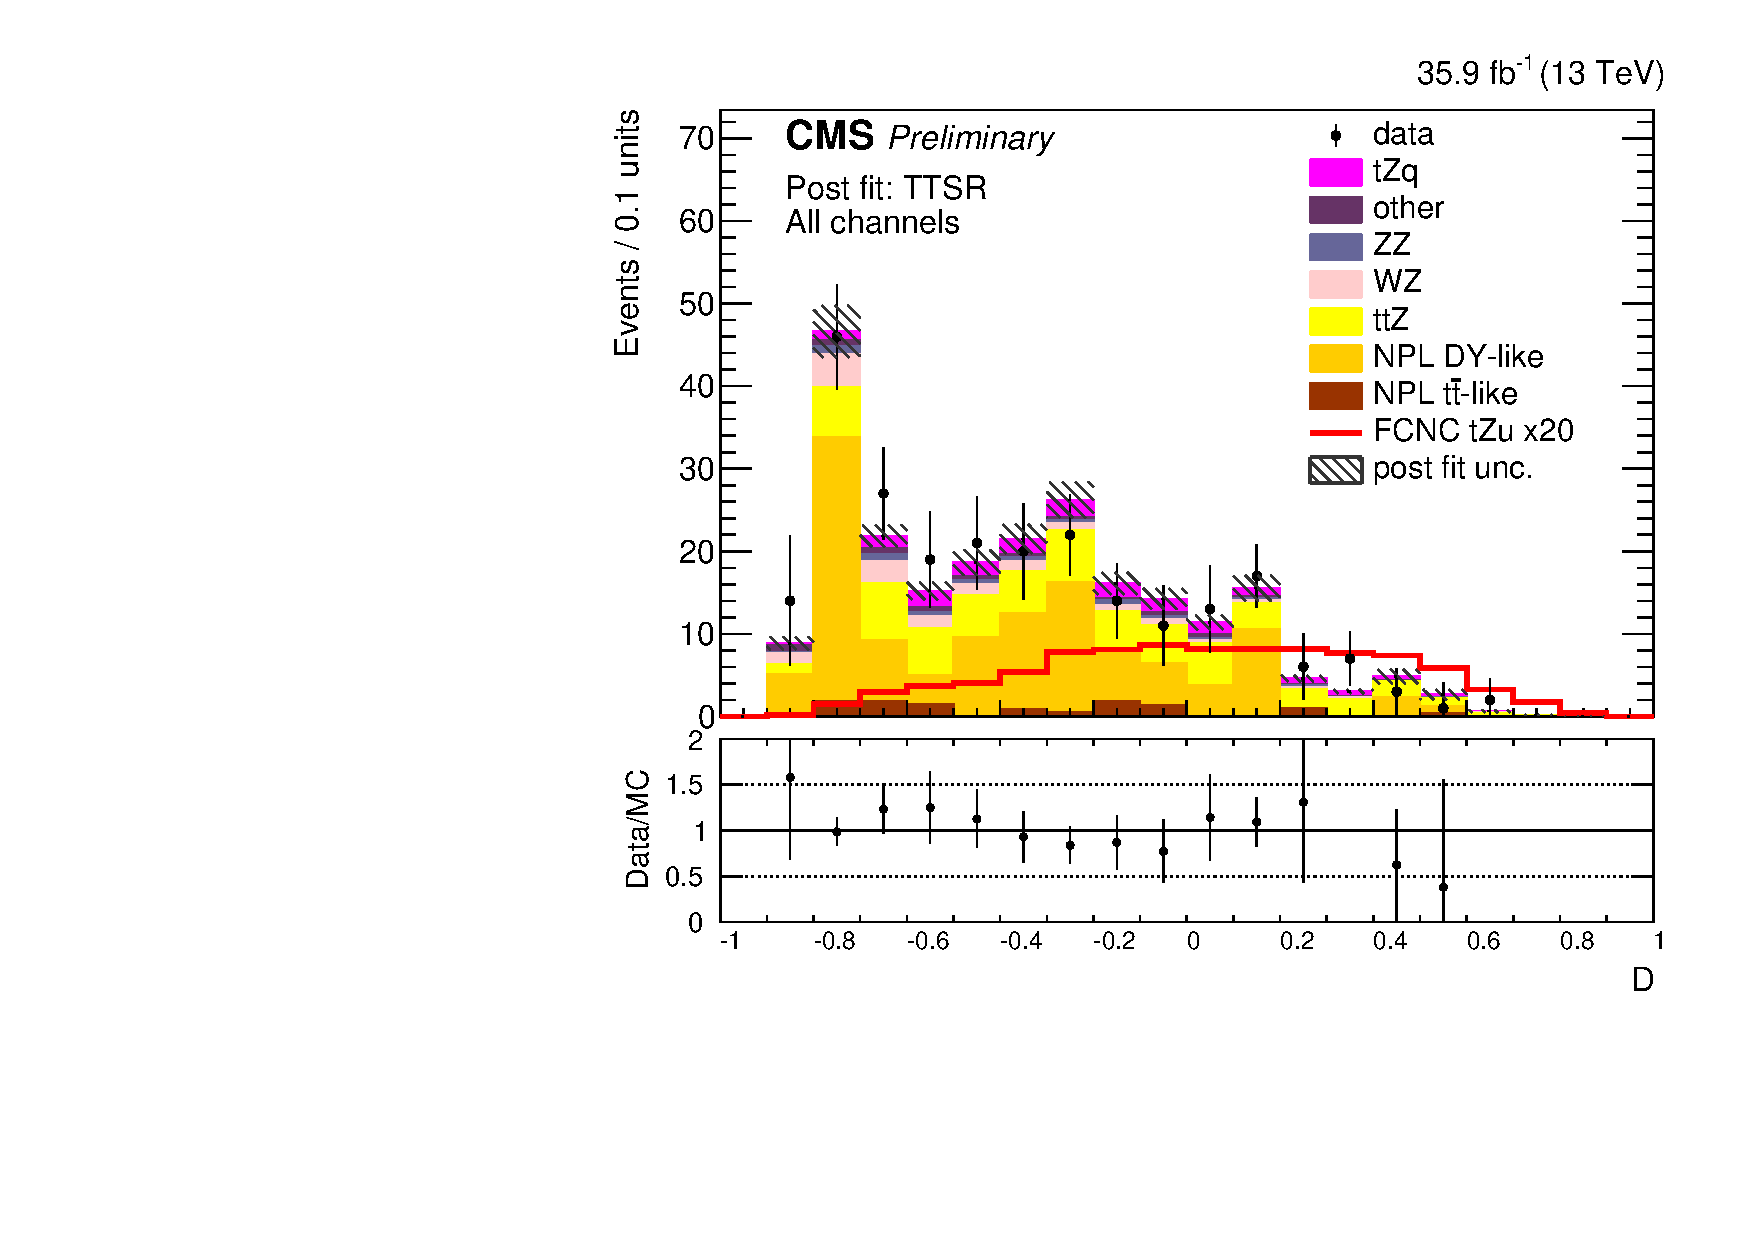
\includegraphics[width=0.45\textwidth]{figures/CMS-PAS-TOP-17-017_Figure_003-a}
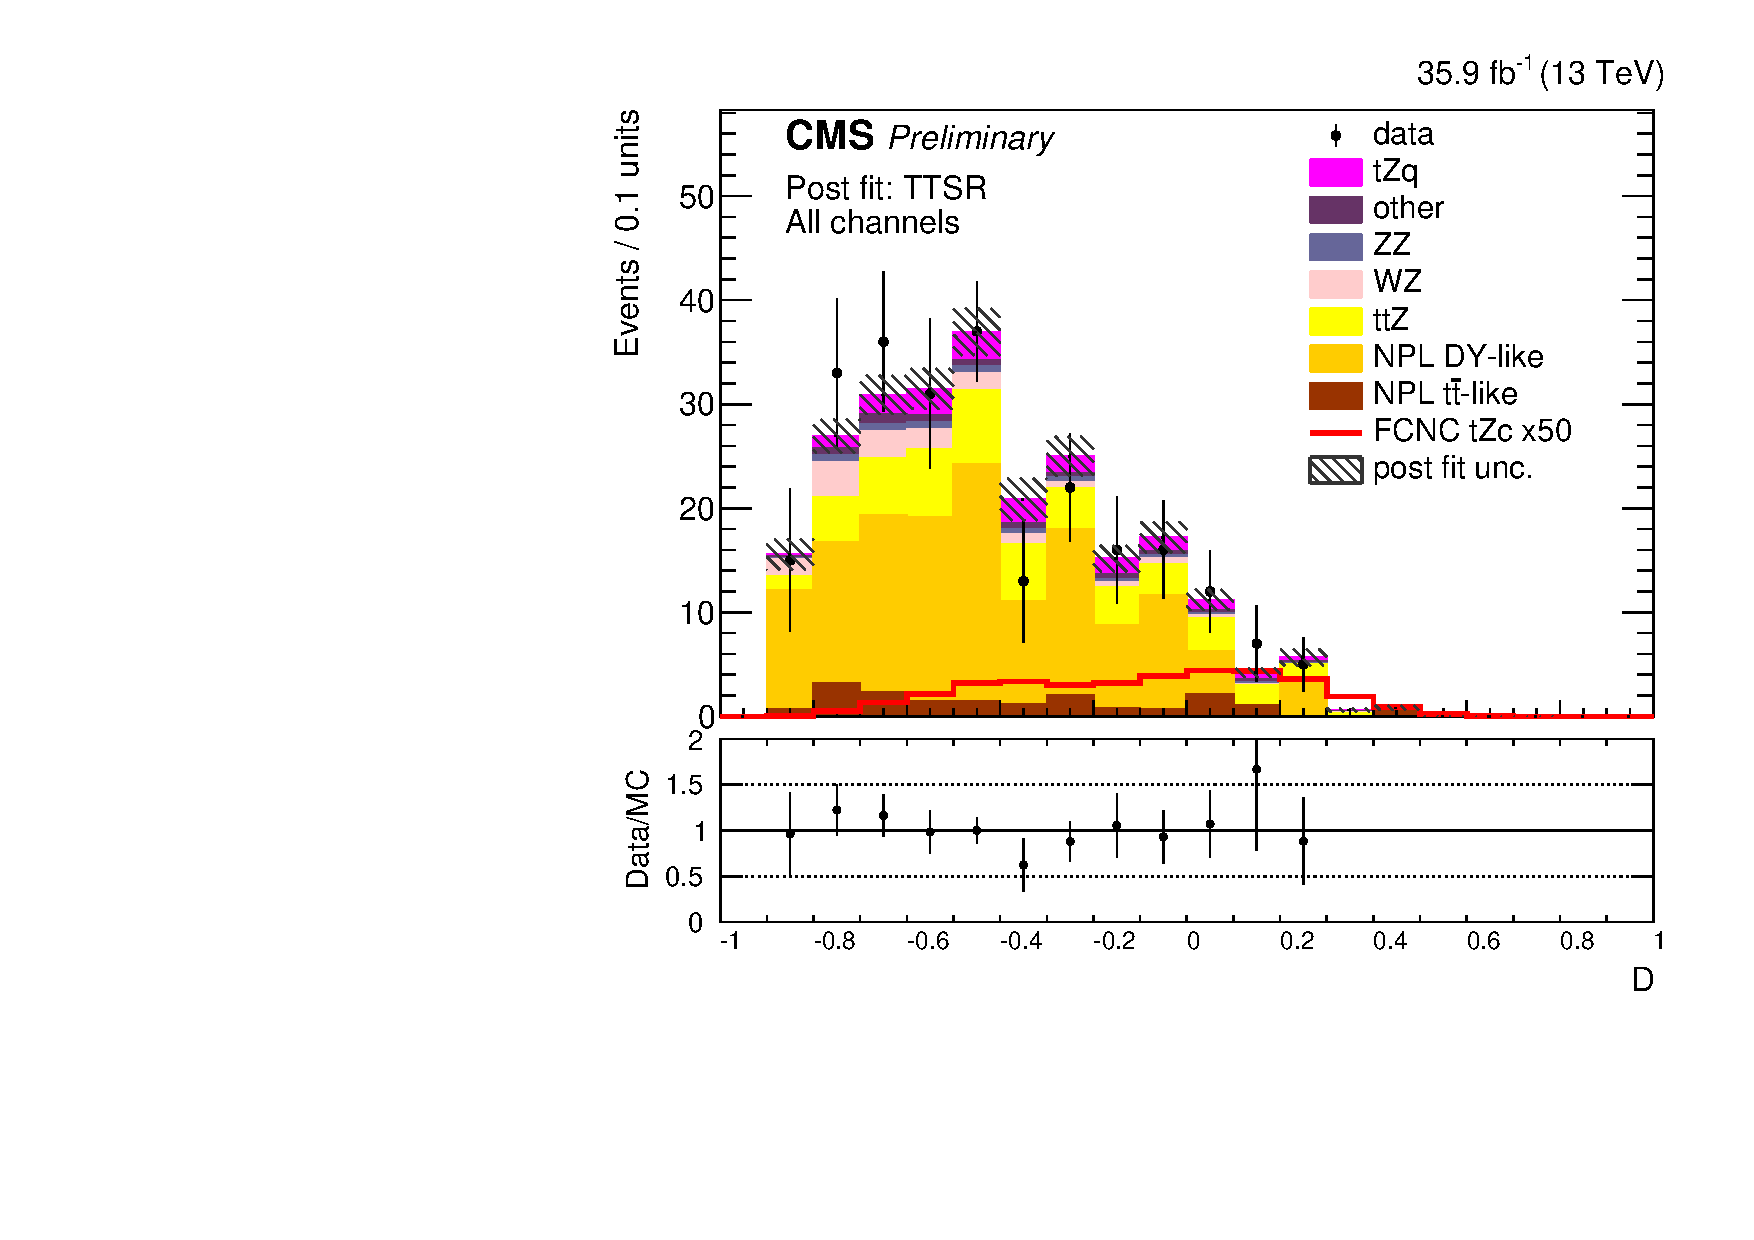
\includegraphics[width=0.45\textwidth]{figures/CMS-PAS-TOP-17-017_Figure_003-b}\\
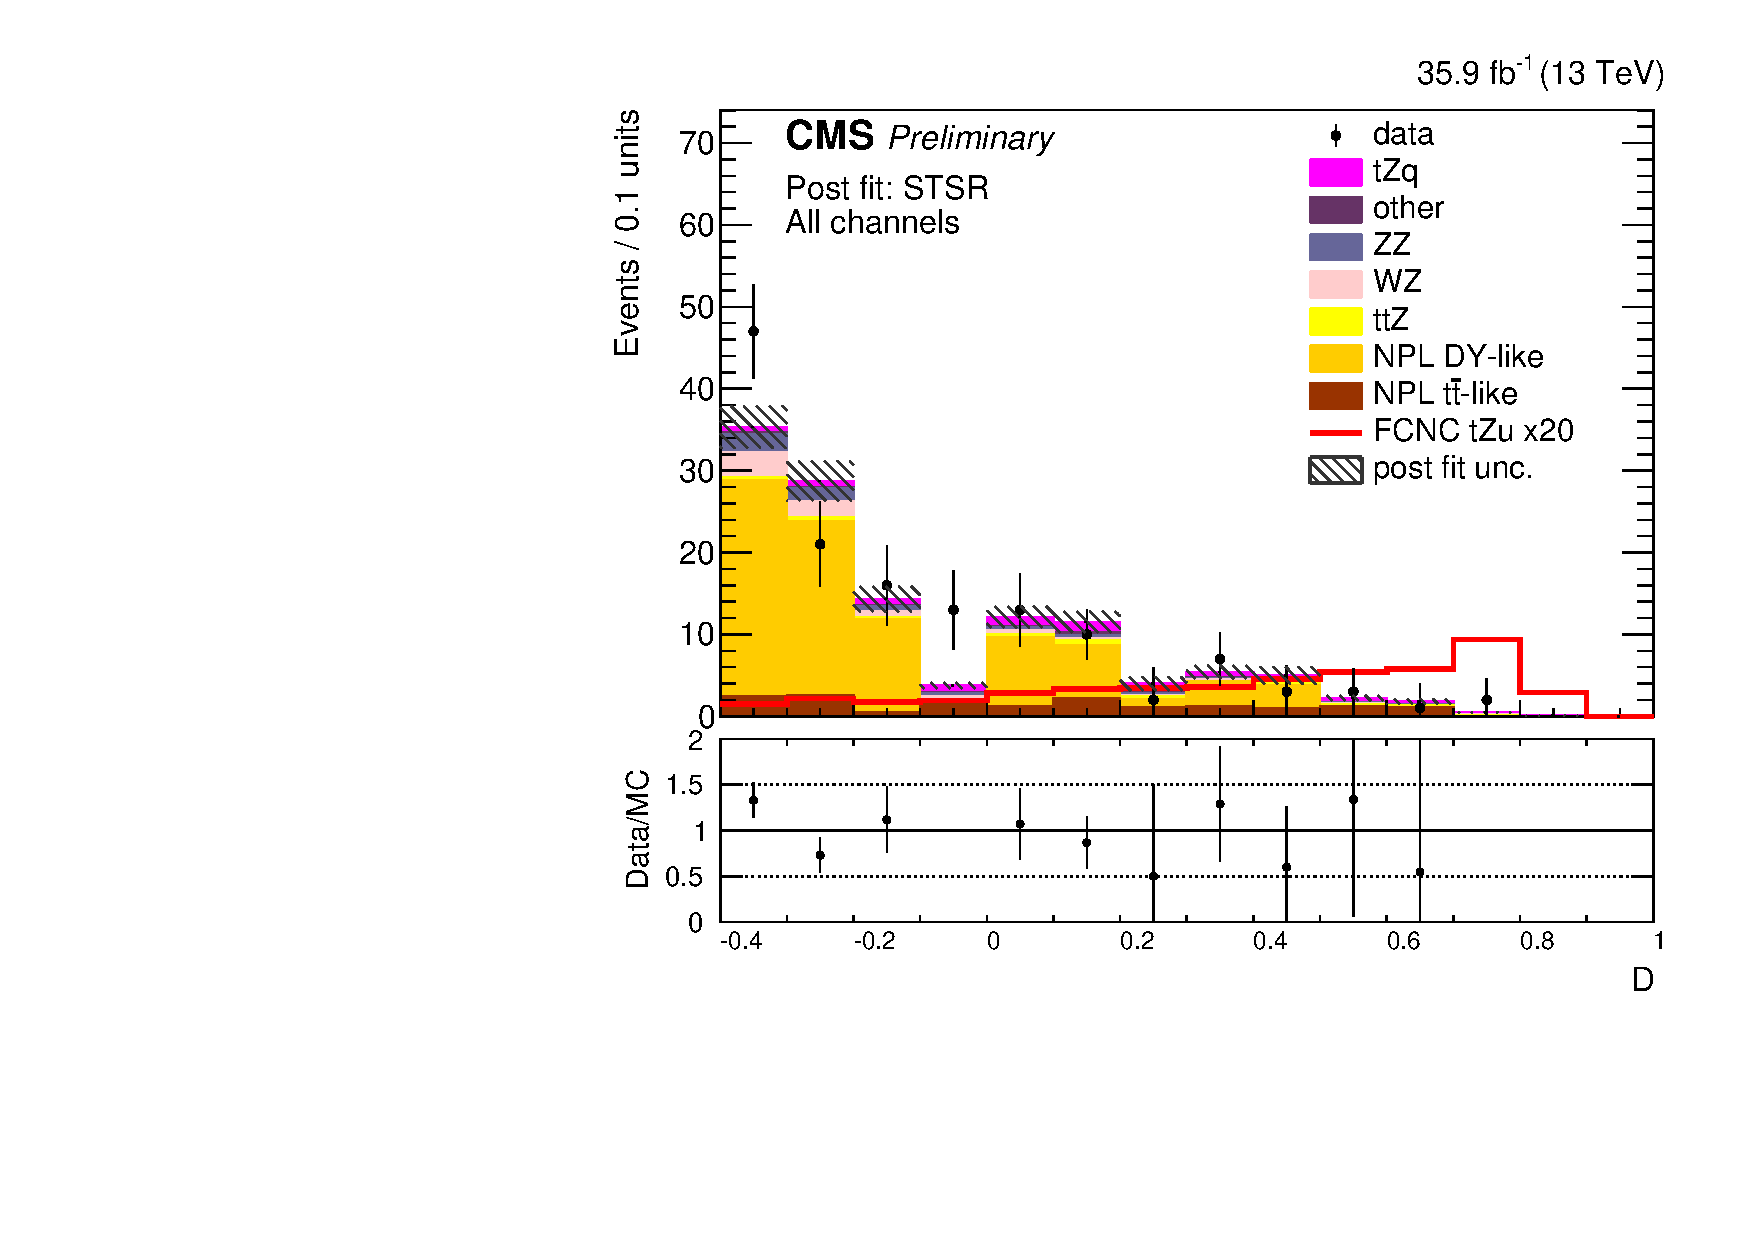
\includegraphics[width=0.45\textwidth]{figures/CMS-PAS-TOP-17-017_Figure_003-c}
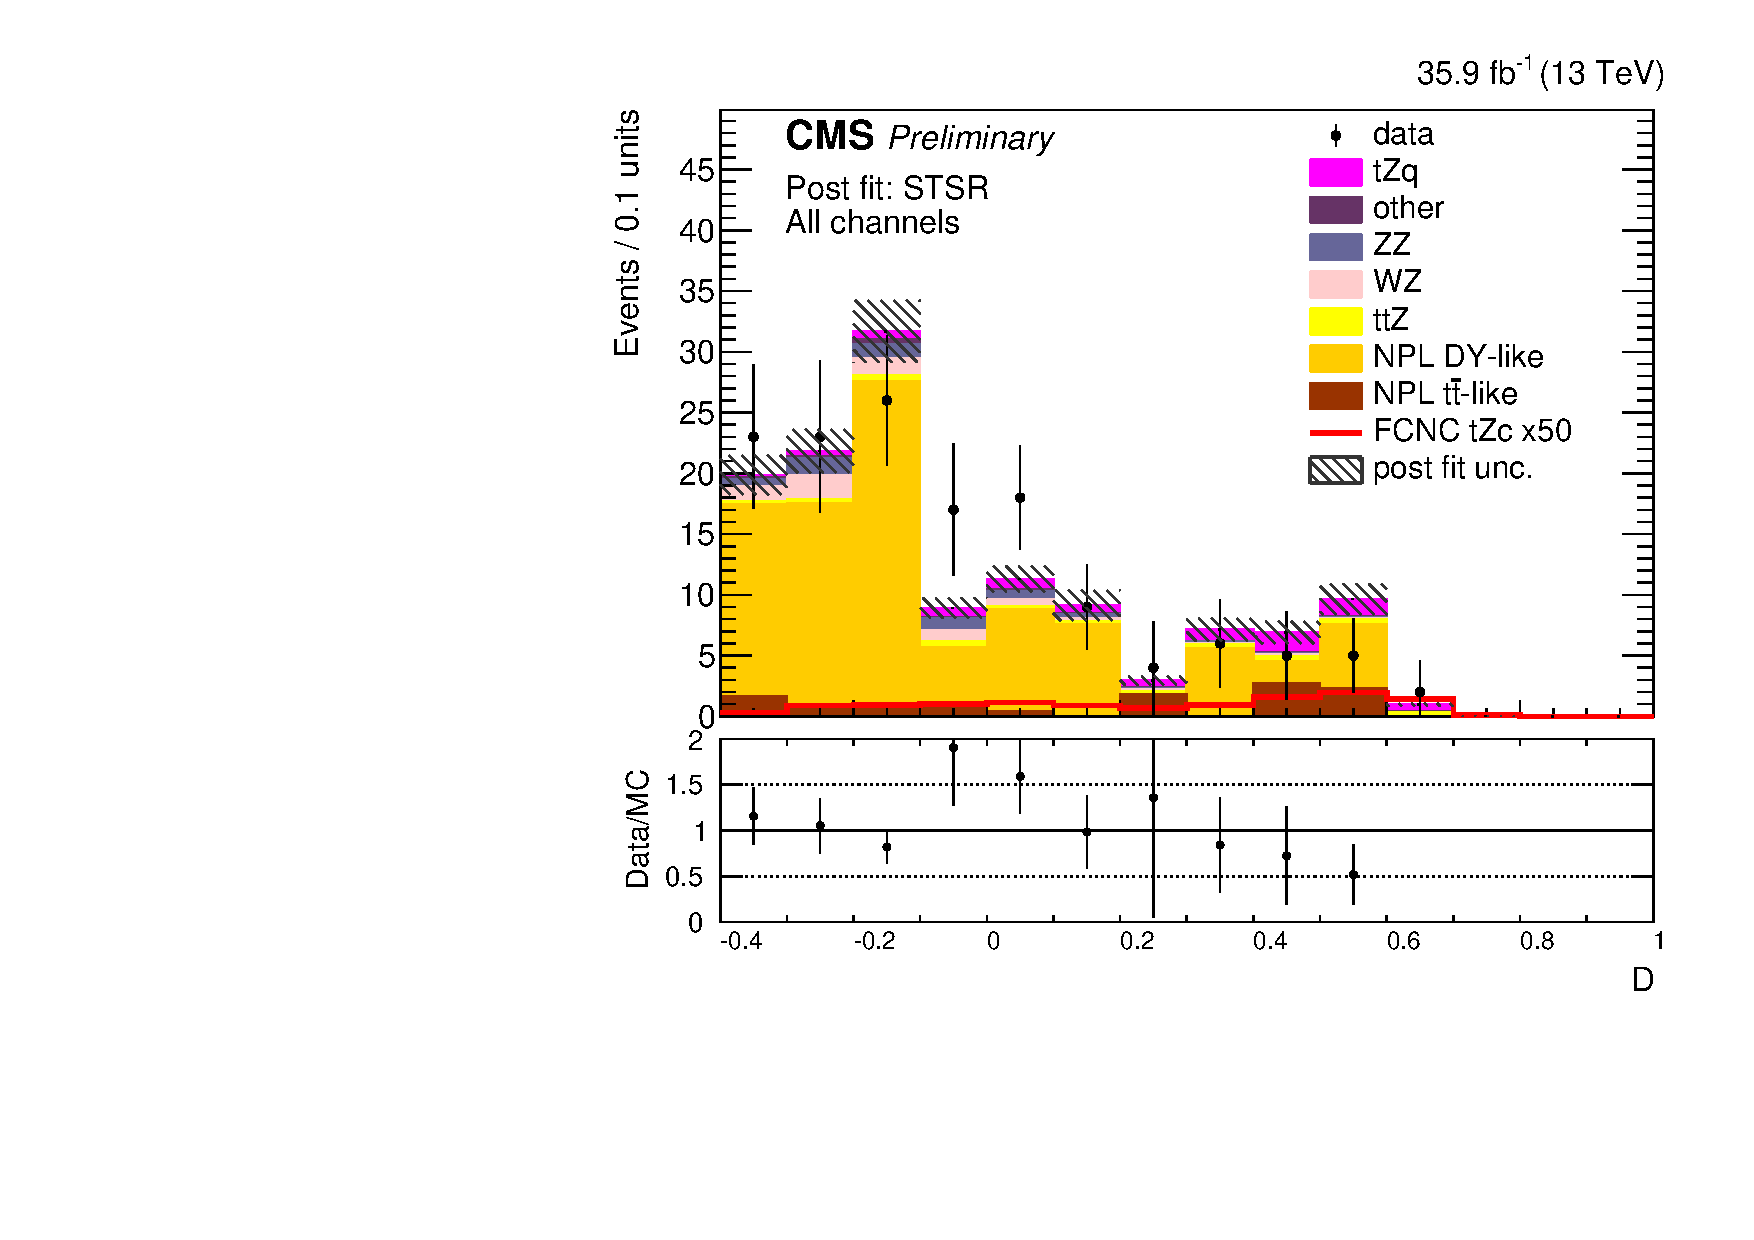
\includegraphics[width=0.45\textwidth]{figures/CMS-PAS-TOP-17-017_Figure_003-d}
\caption{
  The discriminating variable distribution after the fit for all different
  leptonic channels~\cite{top-17-017}. Upper left: top quark pair tZu; upper
  right: top quark pair tZc; lower left: single top quark tZu; lower right:
  single top quark tZc.
}
\label{fig:TOP-17-017_Figure_003}
\end{figure}


\begin{figure}[htb]
\centering
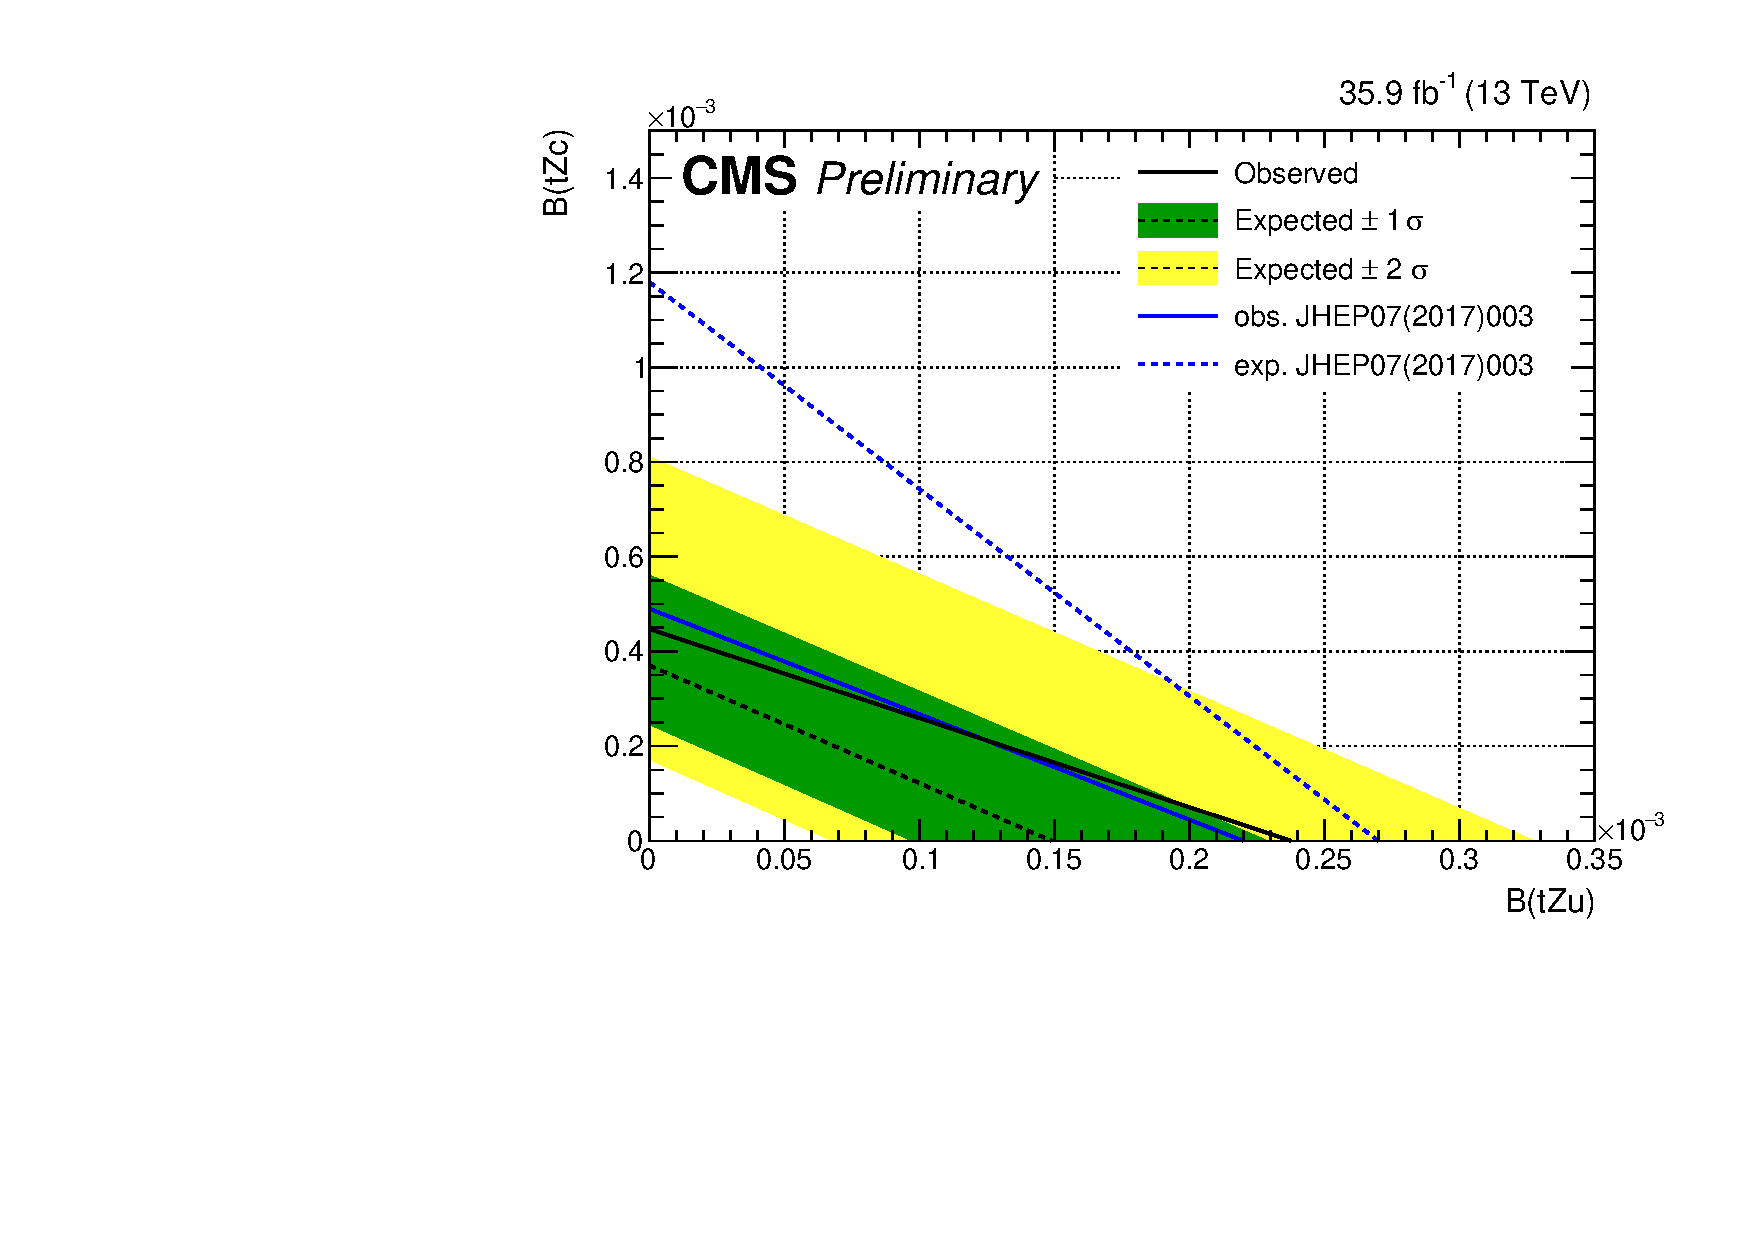
\includegraphics[width=0.45\textwidth]{figures/CMS-PAS-TOP-17-017_Figure_007-a-fixed}
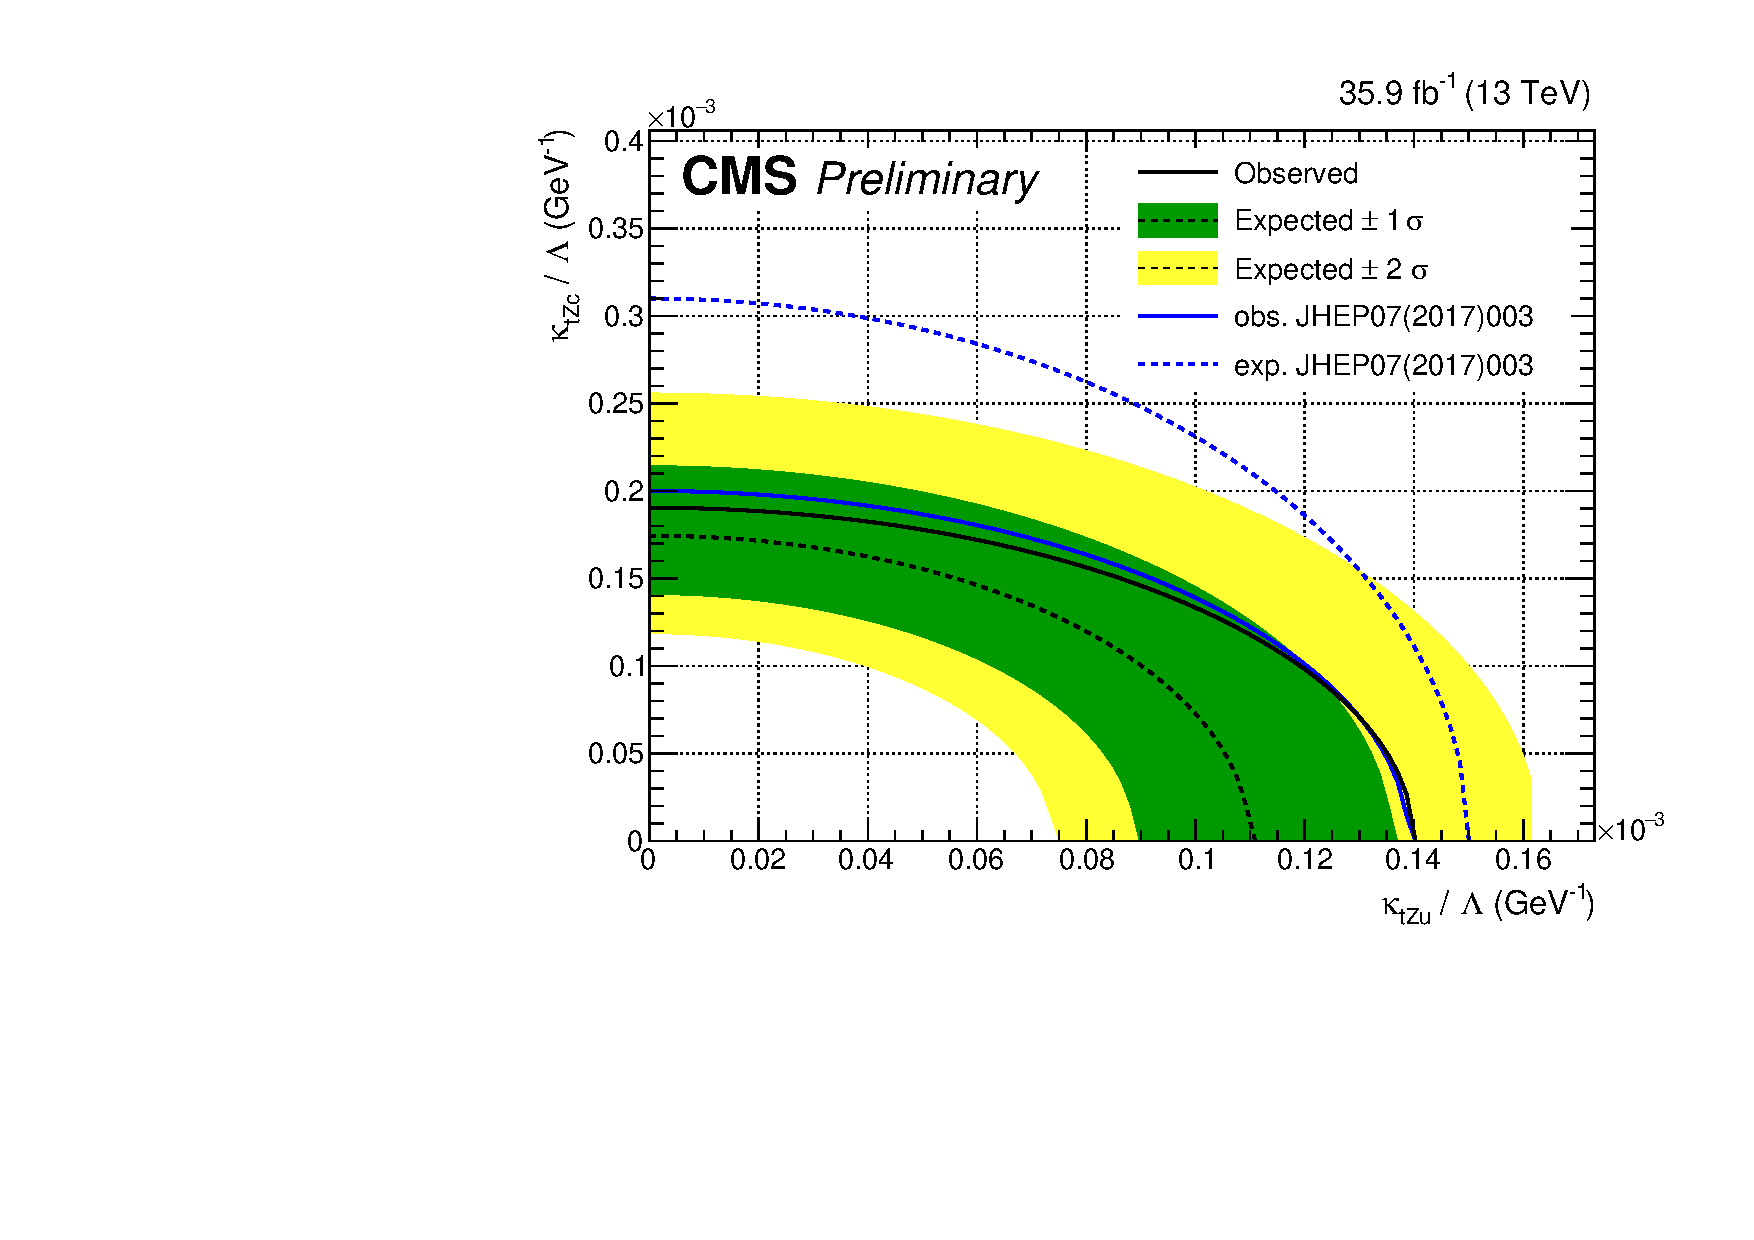
\includegraphics[width=0.45\textwidth]{figures/CMS-PAS-TOP-17-017_Figure_007-b}
\caption{
  Exclusion regions at 95\% CL on the FCNC branching fractions (left)
  and couplings (right) in the 2D plane of both the tZu and tZc
  variables~\cite{top-17-017}. The CMS 8 TeV observed (expected)
  limit is given with a blue line (dashed line).
}
\label{fig:TOP-17-017_Figure_007}
\end{figure}


%-------------------------------------------------------------------------------
\section{FCNC in ${\rm tH \to bb}$}
%-------------------------------------------------------------------------------

In this analysis~\cite{top-17-003} we search for FCNC in events with the
top quark and the Higgs boson, but considering only the Higgs boson decays to b
quarks. The tH FCNC interaction is studied in two channels: the associated
production of a single top quark with the Higgs boson (ST), and the FCNC decays
of top quarks in ${\rm t{\bar t}}$ semileptonic events (TT). As before, the data
sample corresponds to an integrated luminosity of~${\rm 35.9~fb^{-1}}$. Events
with exactly one isolated lepton (electron or muon) are selected, and at least
3 jets are required to be present. As signal events contain three b quarks,
we require that at least two jets are identified as b quark jets by the combined
secondary vertex (CSV) b-tagging algorithm. In order to optimize the sensitivity
to the signal event selection, events are split into five categories based on
the total number of reconstructed jets and on the number of b-tagged jets.
Using the energy and momenta of all particles, a full kinematic reconstruction
of the event is performed for several signal (ST and TT) and background
(${\rm t{\bar t}}$) hypotheses. The reconstruction is performed for all possible
permutations of the b-tagged jets to be associated with the decay products of
the Higgs boson or the top quark. The reconstructed kinematic variables for each
permutation are inputs for a multivariate analysis that uses a BDT, trained
to distinguish the correct from the wrong b jet assignments. In addition,
kinematic variables from the event reconstruction are used to construct several
BDTs to suppress backgrounds. The BDTs are trained for each jet multiplicity
category to identify signal events that are generated either for
${\rm \kappa_{Hut}}$ (Hut) or ${\rm \kappa_{Hct}}$ (Hct) coupling against the
sum of all background events. Separate trainings of the BDT for Hut and Hct are
done. Distributions for some of the most discriminating BDT input variables,
in the category with three jets, all of them b-tagged, can be seen in
Figure~\ref{fig:TOP-17-003_Figure_002}. The final observable used to extract
signal events is defined as the BDT score distribution. The resultant observed
(expected) 95\% CL exclusion limits on top quark FCNC decay branching fractions
are ${\cal B}({\rm t \to uH}) < 0.47\%~(0.34\%)$ and
${\cal B}({\rm t \to cH}) < 0.47\%~(0.44\%)$. Two-dimensional limits are also
shown in Figure~\ref{fig:TOP-17-003_Figures_006-007}. We define a signal strength
parameter $\mu = \sigma/\sigma_{\rm sig}$, where $\sigma$ is the cross section
excluded at 95\% CL and $\sigma_{\rm sig}$ is the predicted cross section for
signal. A maximum likelihood fit is performed for the signal strength, and is
shown in Figure~\ref{fig:TOP-17-003_Figures_006-007}.


\begin{figure}[htb]
\centering
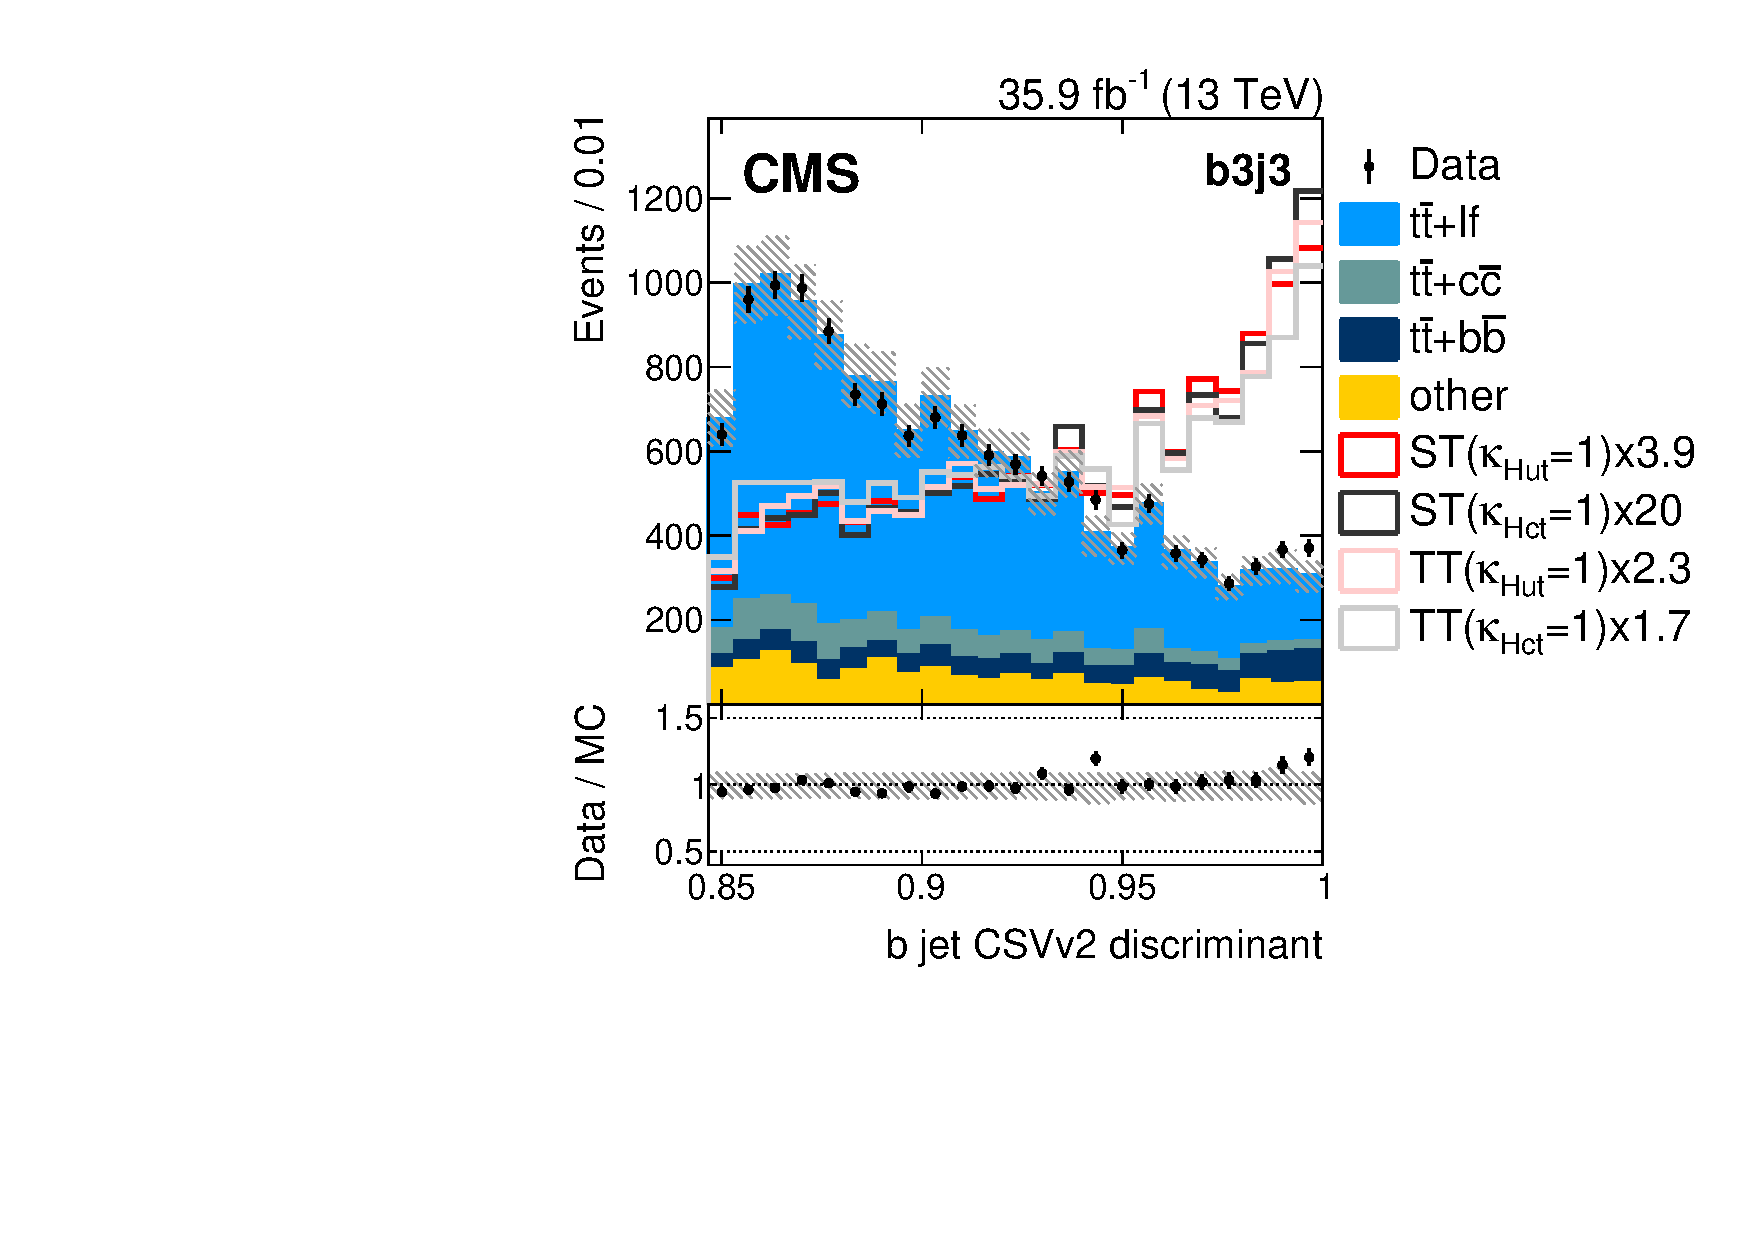
\includegraphics[width=0.45\textwidth]{figures/CMS-TOP-17-003_Figure_002-b}
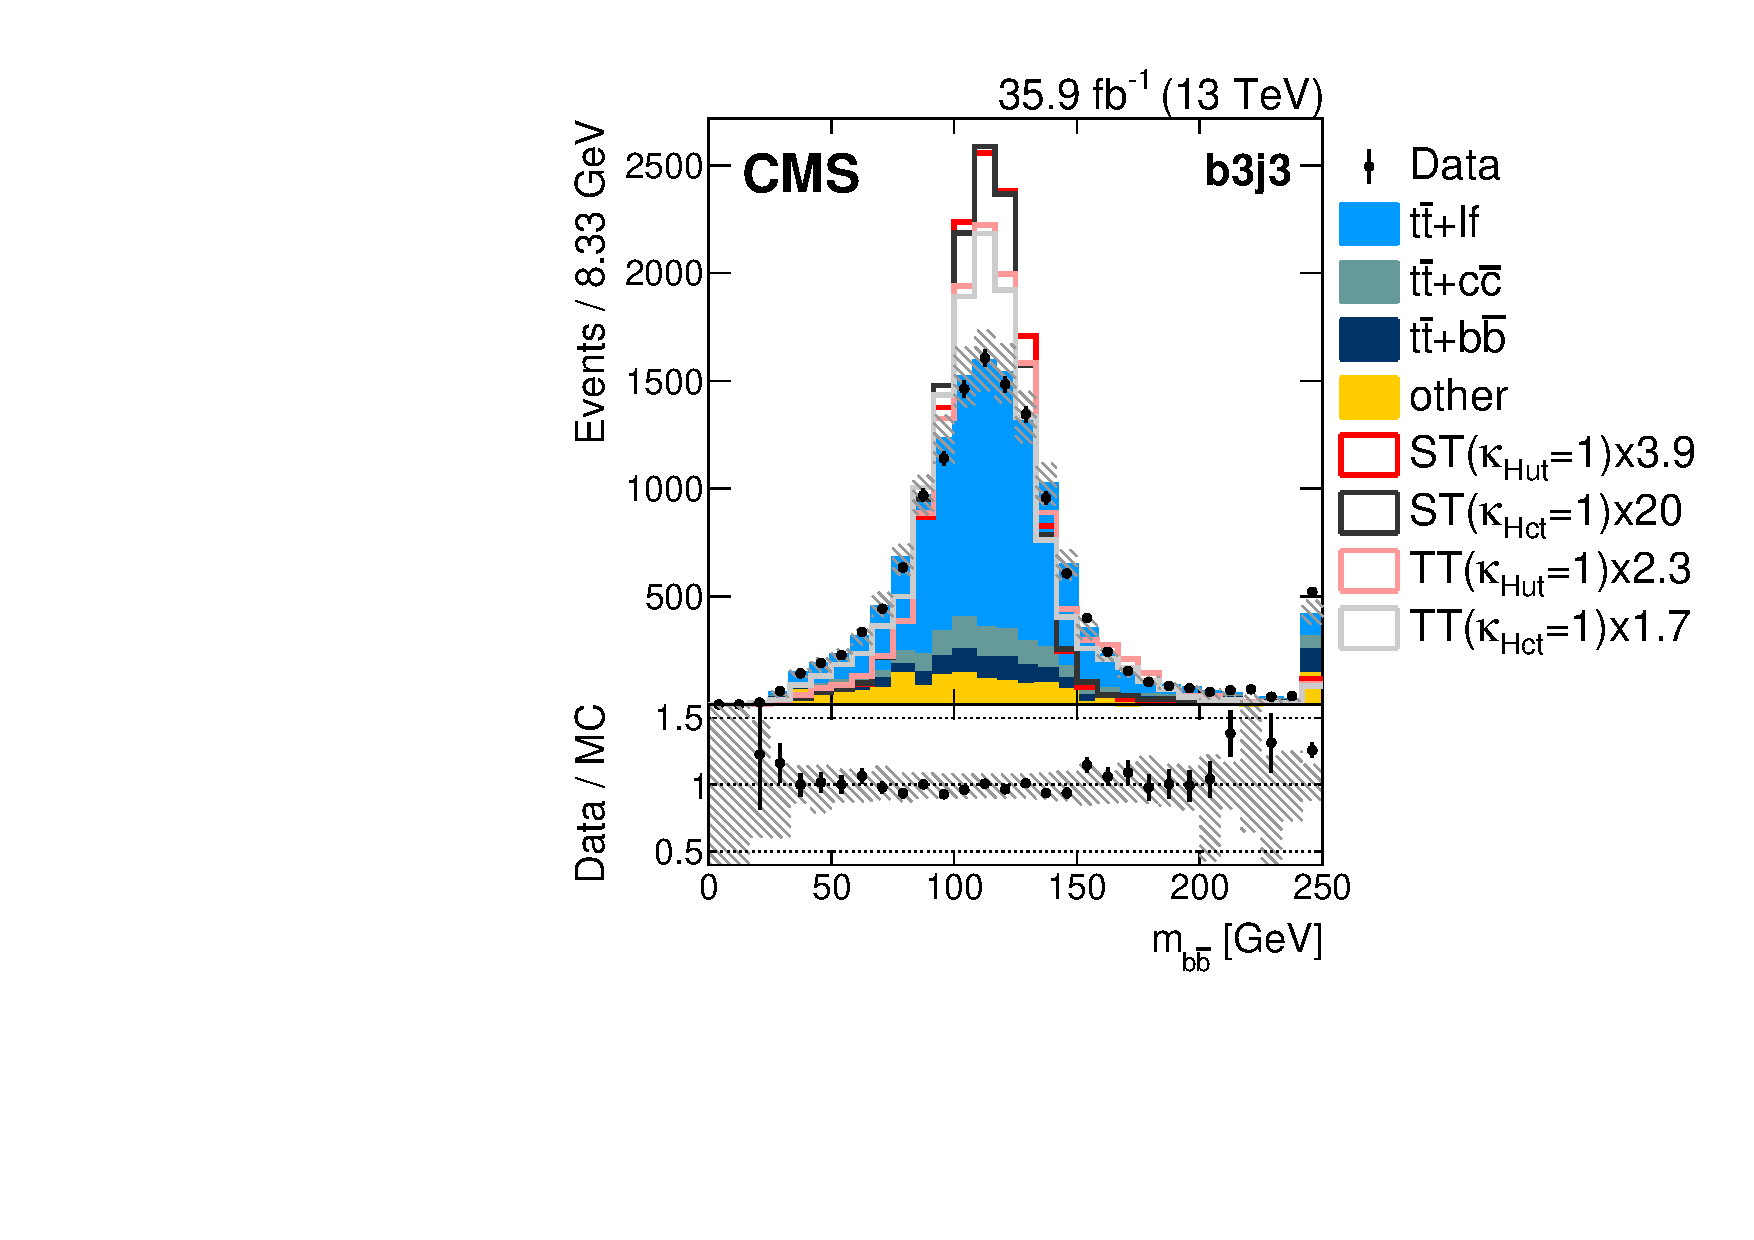
\includegraphics[width=0.45\textwidth]{figures/CMS-TOP-17-003_Figure_002-c}
\caption{
  Comparison between data and simulation for some of the most discriminating
  BDT input variables in the category with three jets, all of them
  b-tagged~\cite{top-17-003}: CSV discriminant value for one of the
  reconstructed b jets assigned to Higgs boson decay (left), and reconstructed
  invariant mass of two b jets associated with the Higgs boson decay (right).
}
\label{fig:TOP-17-003_Figure_002}
\end{figure}


\begin{figure}[htb]
\centering
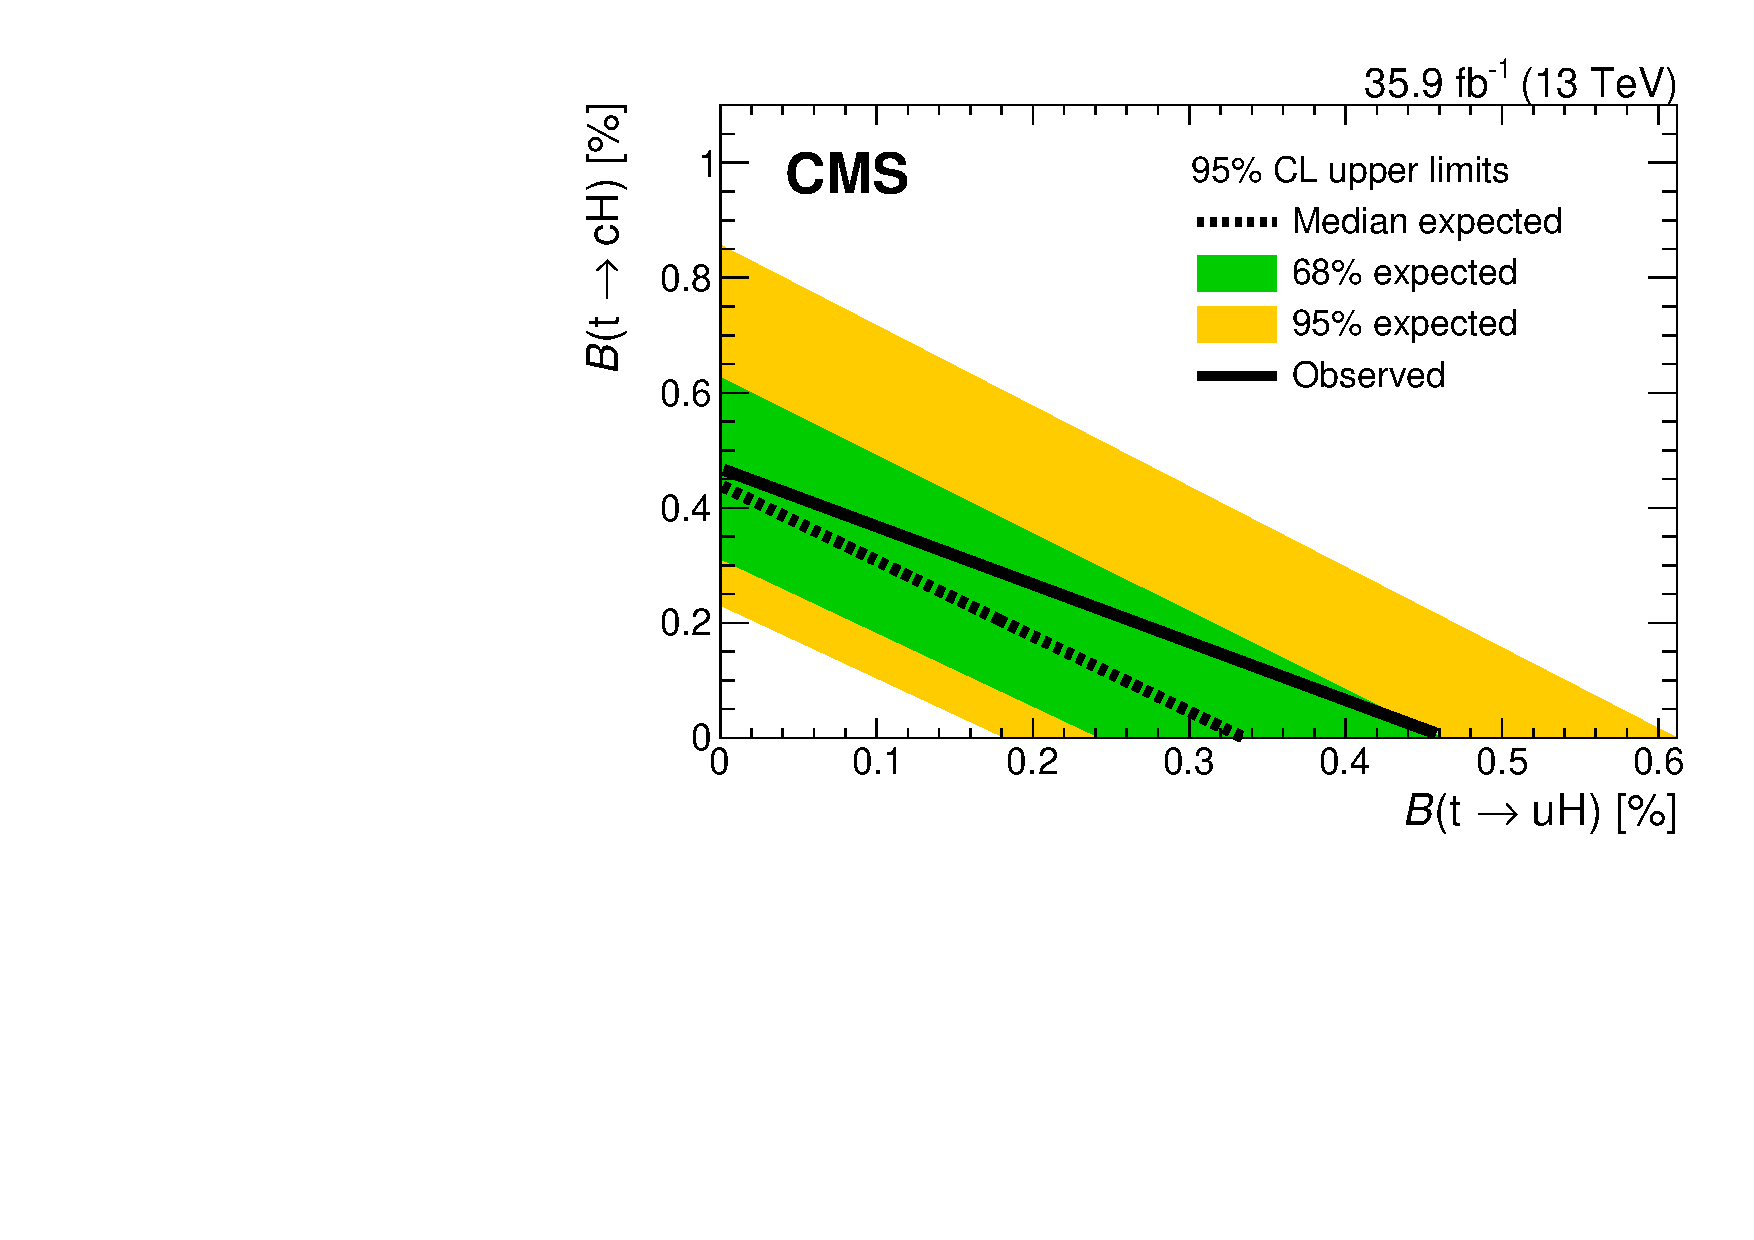
\includegraphics[width=0.45\textwidth]{figures/CMS-TOP-17-003_Figure_006}\\
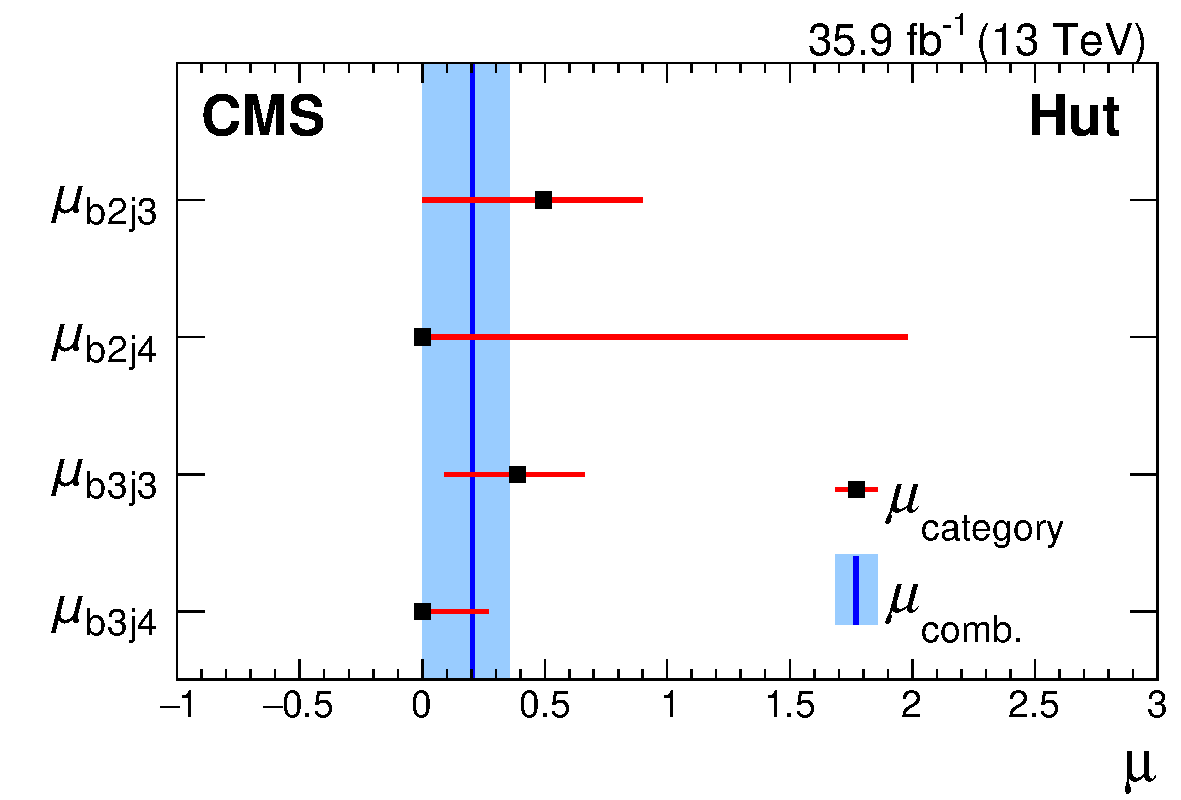
\includegraphics[width=0.45\textwidth]{figures/CMS-TOP-17-003_Figure_007-a}
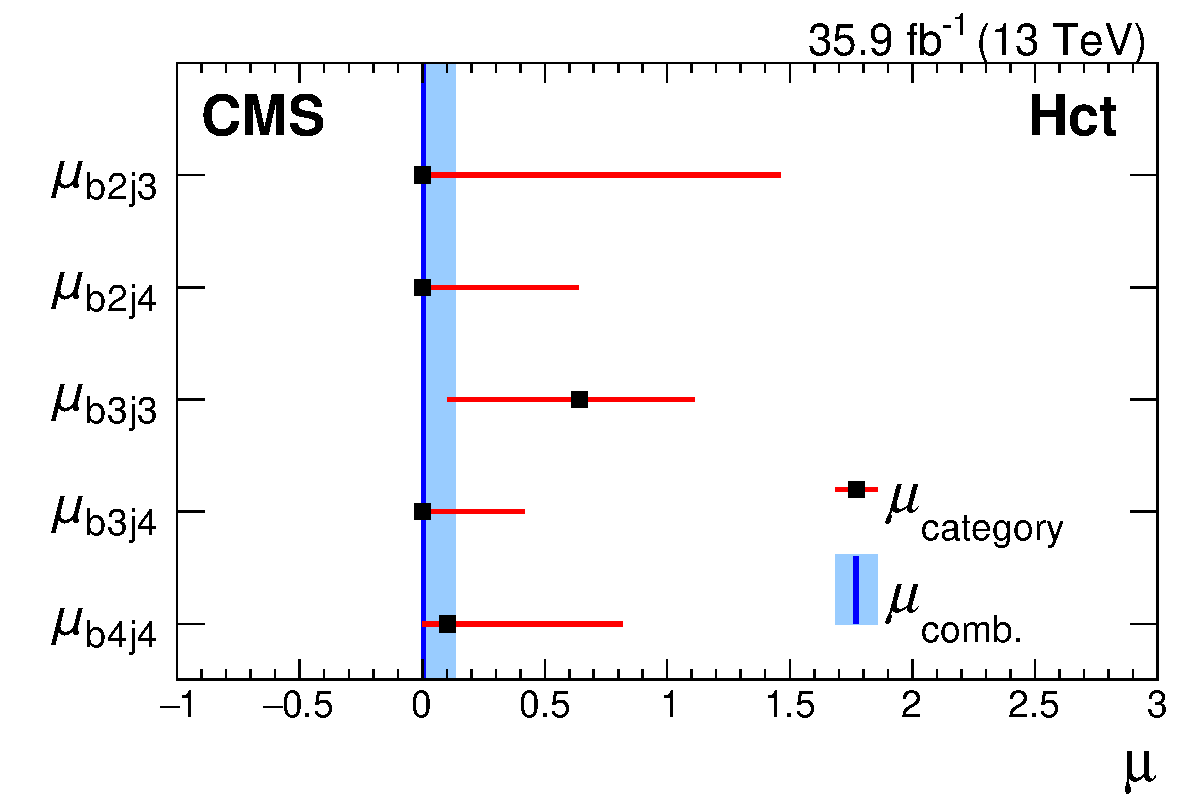
\includegraphics[width=0.45\textwidth]{figures/CMS-TOP-17-003_Figure_007-b}
\caption{
  Upper limits on ${\cal B}({\rm t \to uH})$ and ${\cal B}({\rm t \to cH})$ at
  95\% CL (top), and the best fit signal strength for Hut (bottom left) and Hct
  (bottom right), which is restricted to positive values in the
  fit~\cite{top-17-003}.
}
\label{fig:TOP-17-003_Figures_006-007}
\end{figure}

A CMS and ATLAS summary~\cite{cms-atlas-fcnc} of the current 95\% CL observed
limits on the branching ratios of the top quark decays via FCNC to a quark and
a neutral boson is shown in Figure~\ref{fig:fcnc_summarybsm_may18}.

\begin{figure}[htb]
\centering
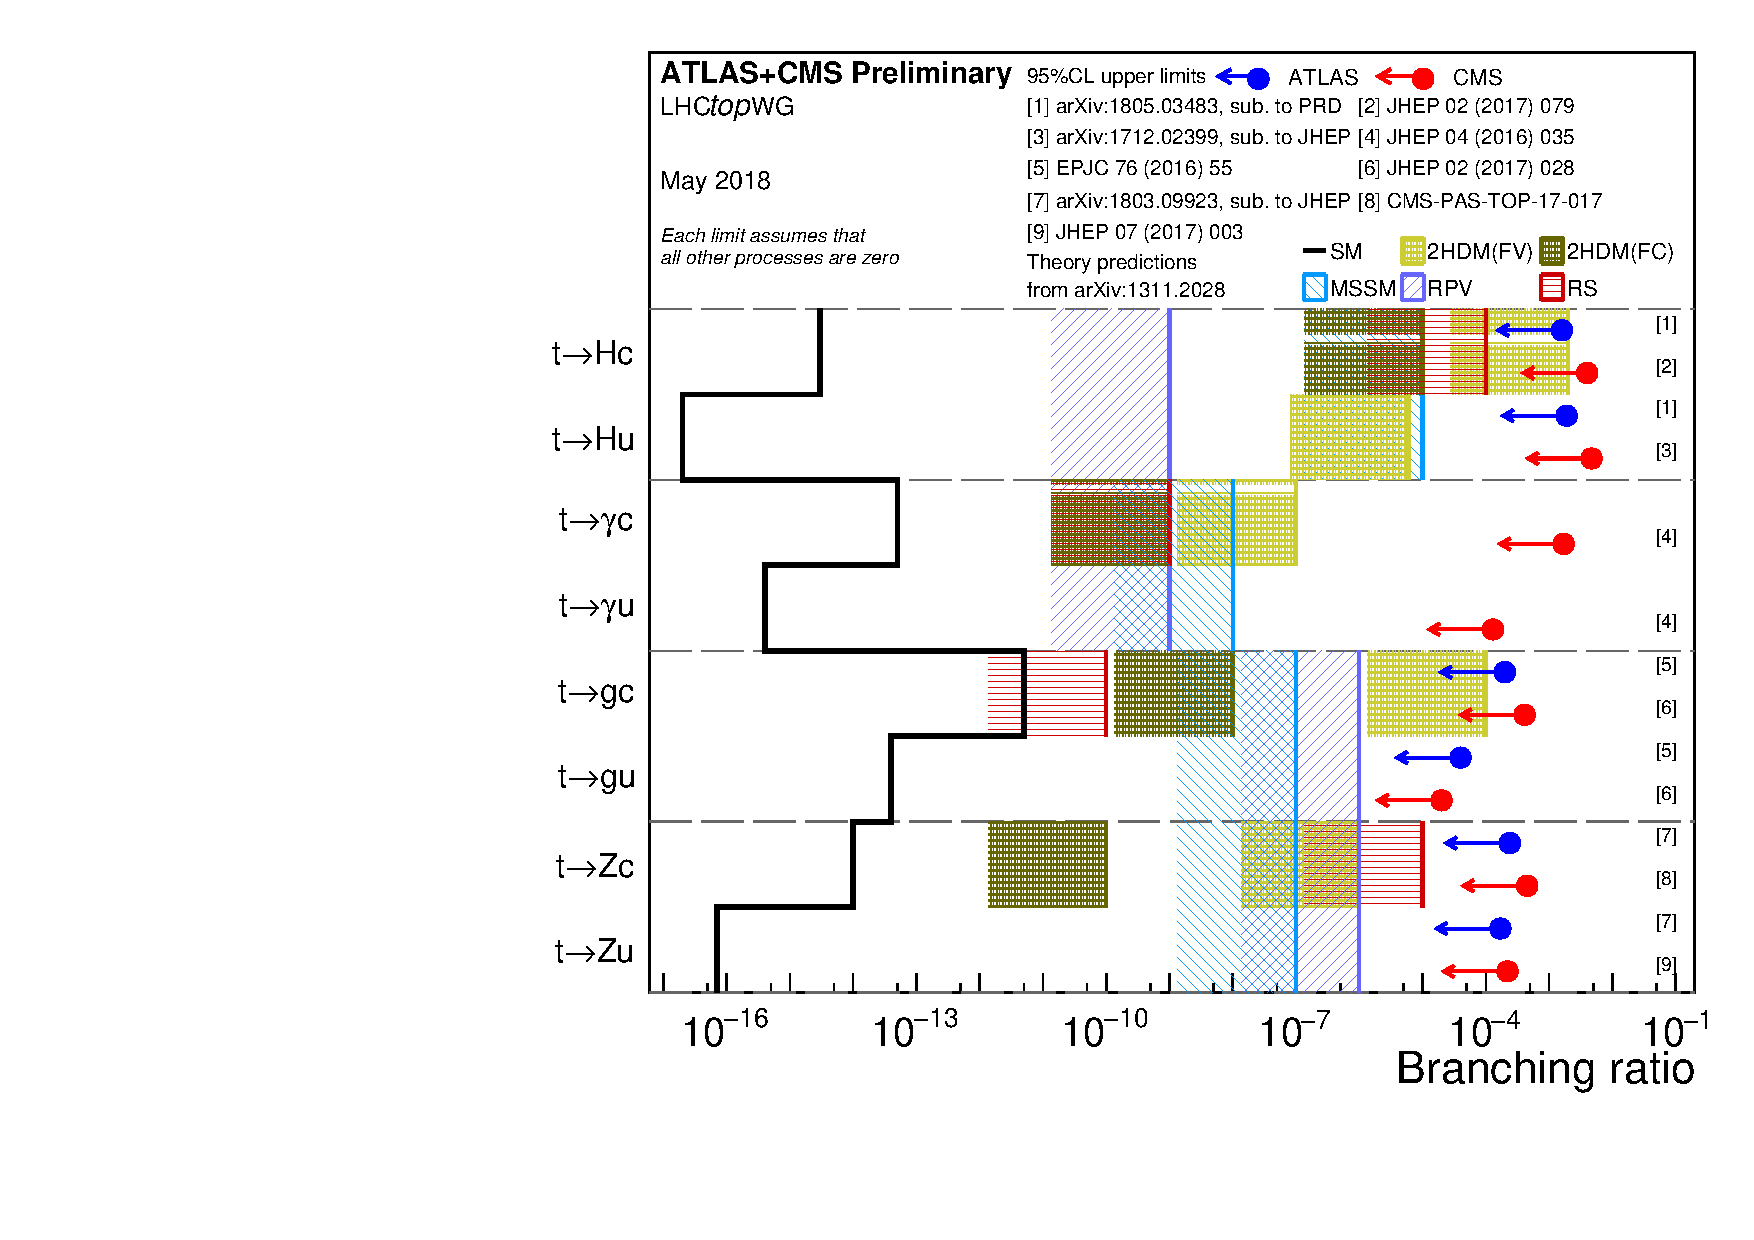
\includegraphics[width=0.6\textwidth]{figures/fcnc_summarybsm_may18}
\caption{
  Summary of the current 95\% confidence level observed limits on the branching
  ratios of the top quark decays via flavour changing neutral currents to a
  quark and a neutral boson by the ATLAS and CMS Collaborations compared to
  several new physics models~\cite{cms-atlas-fcnc}.
}
\label{fig:fcnc_summarybsm_may18}
\end{figure}


%-------------------------------------------------------------------------------
\section{Angular observables in ${\rm B^+ \to K^+\mu^+\mu^-}$}
%-------------------------------------------------------------------------------

In Reference~\cite{bph-15-001} we present a study of the angular distribution of
the FCNC
decay ${\rm B^+ \to K^+\mu^+\mu^-}$ in pp collisions at the center-of-mass
energy of 8~TeV. The analysis is based on data collected by the CMS detector at
the LHC, corresponding to an integrated luminosity of ${\rm 20.5~fb^{-1}}$.
There are two model-independent parameters that describe the decay rate for the
process: the forward/backward asymmetry $A_{FB}$ of the dimuon system and the
contribution $F_H$ from the pseudo-scalar, scalar, and tensor amplitudes to the
decay width. Because SM amplitudes may interefere with the contributions from
non-SM particles inside loop diagrams, this decay channel can probe the presence
of yet unobserved particles and processes.
The decay rate for the process ${\rm B^+ \to K^+\mu^+\mu^-}$ depends on
$\cos\theta_{\ell}$, where $\theta_{\ell}$ is the angle between the direction
of the $\mu^-$ and the ${\rm K^+}$ in the dilepton rest frame. The
$\cos\theta_{\ell}$-dependence of the decay process can be parametrized in
terms of the observables of interest $A_{FB}$ and $F_H$, which are extracted
with an extended unbinned maximum-likelihood fit to the angular distributions
of the selected B candidates in the data, in bins of $q^2$.
Figure~\ref{fig:BPH-15-001_Figures_003-004} shows the projections from the
two-dimensional fits for the inclusive low-$q^2$ range ${\rm 1-6~GeV^2}$.
The measured values of $A_{FB}$ and $F_H$ for each $q^2$ bin are shown in
Figure~\ref{fig:BPH-15-001_Figure_005__BPH-15-008_Figure003}
(top distributions). The results are consistent with previous measurements and
with various standard model predictions.


\begin{figure}[htb]
\centering
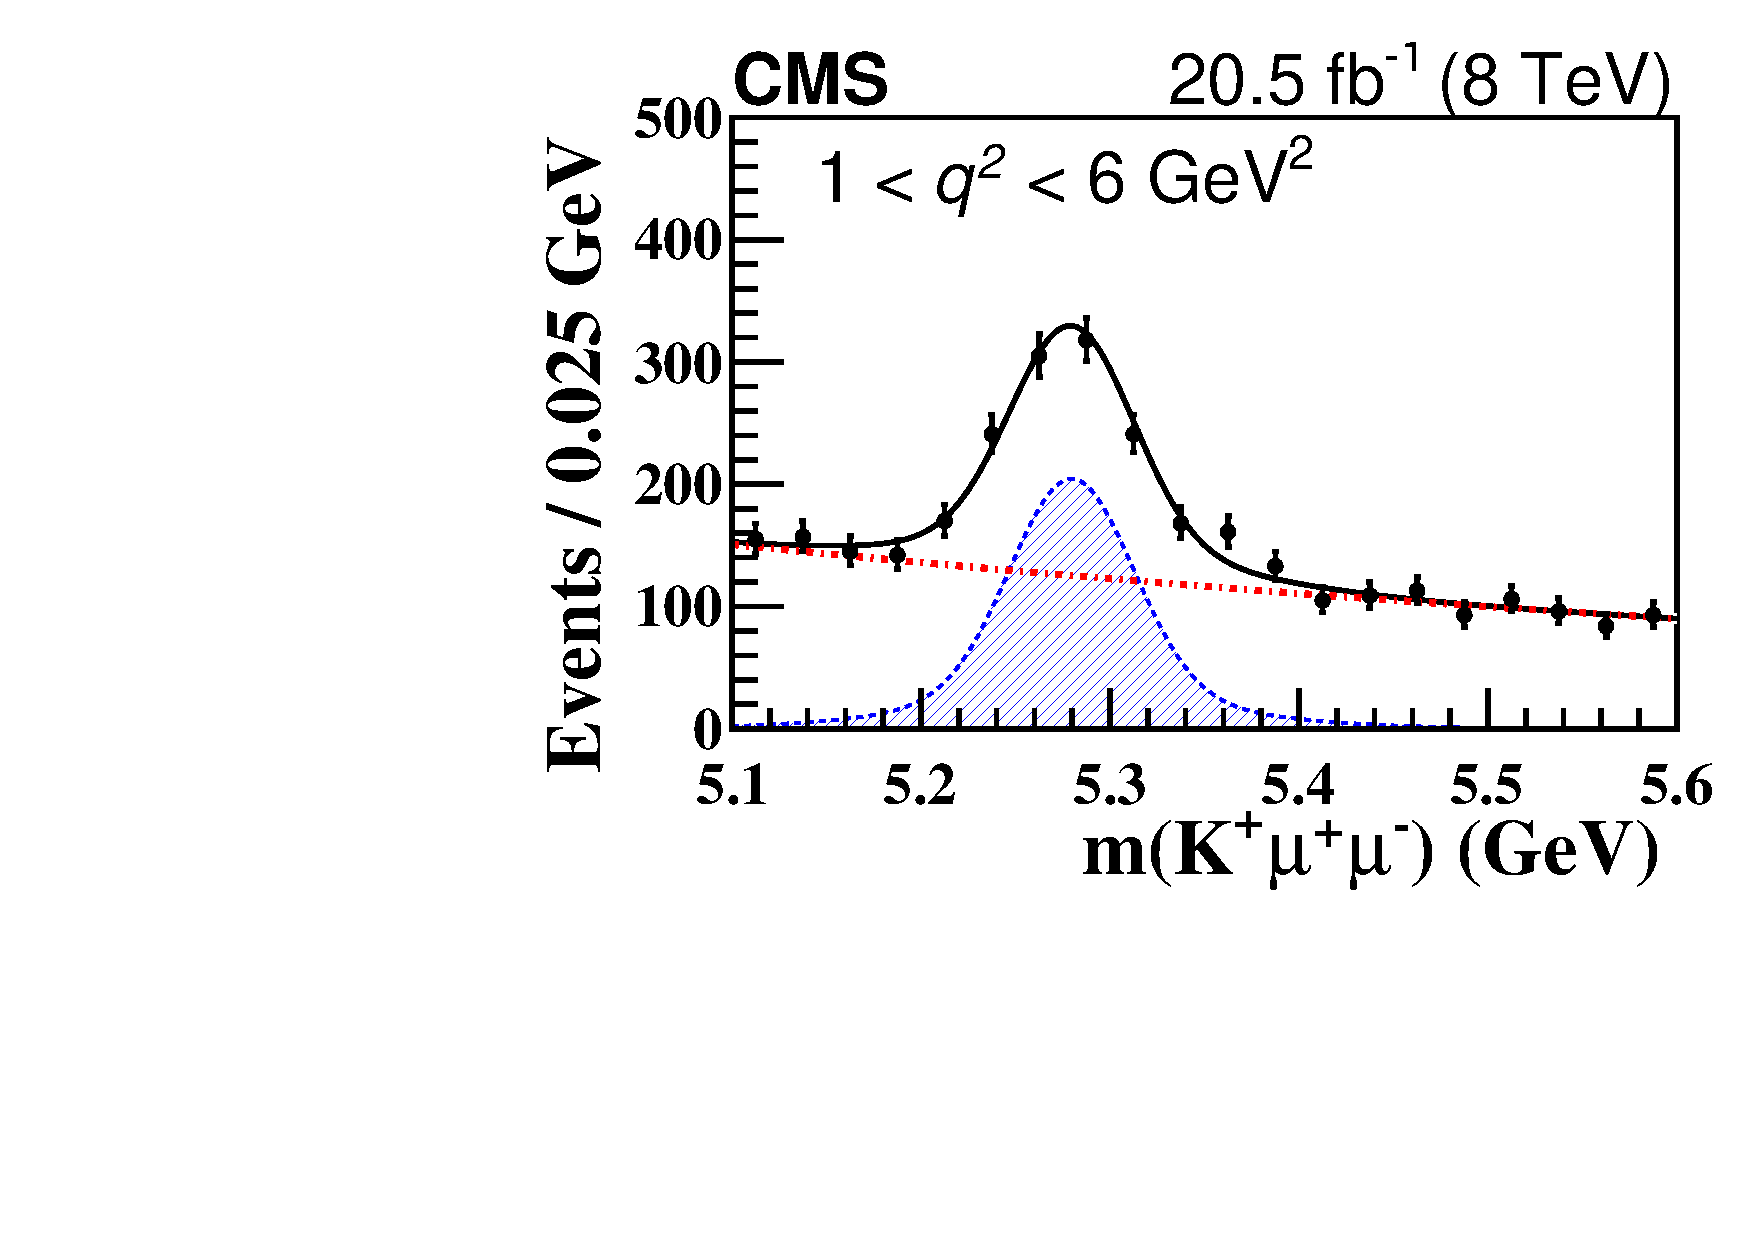
\includegraphics[width=0.45\textwidth]{figures/CMS-BPH-15-001_Figure_003-h}
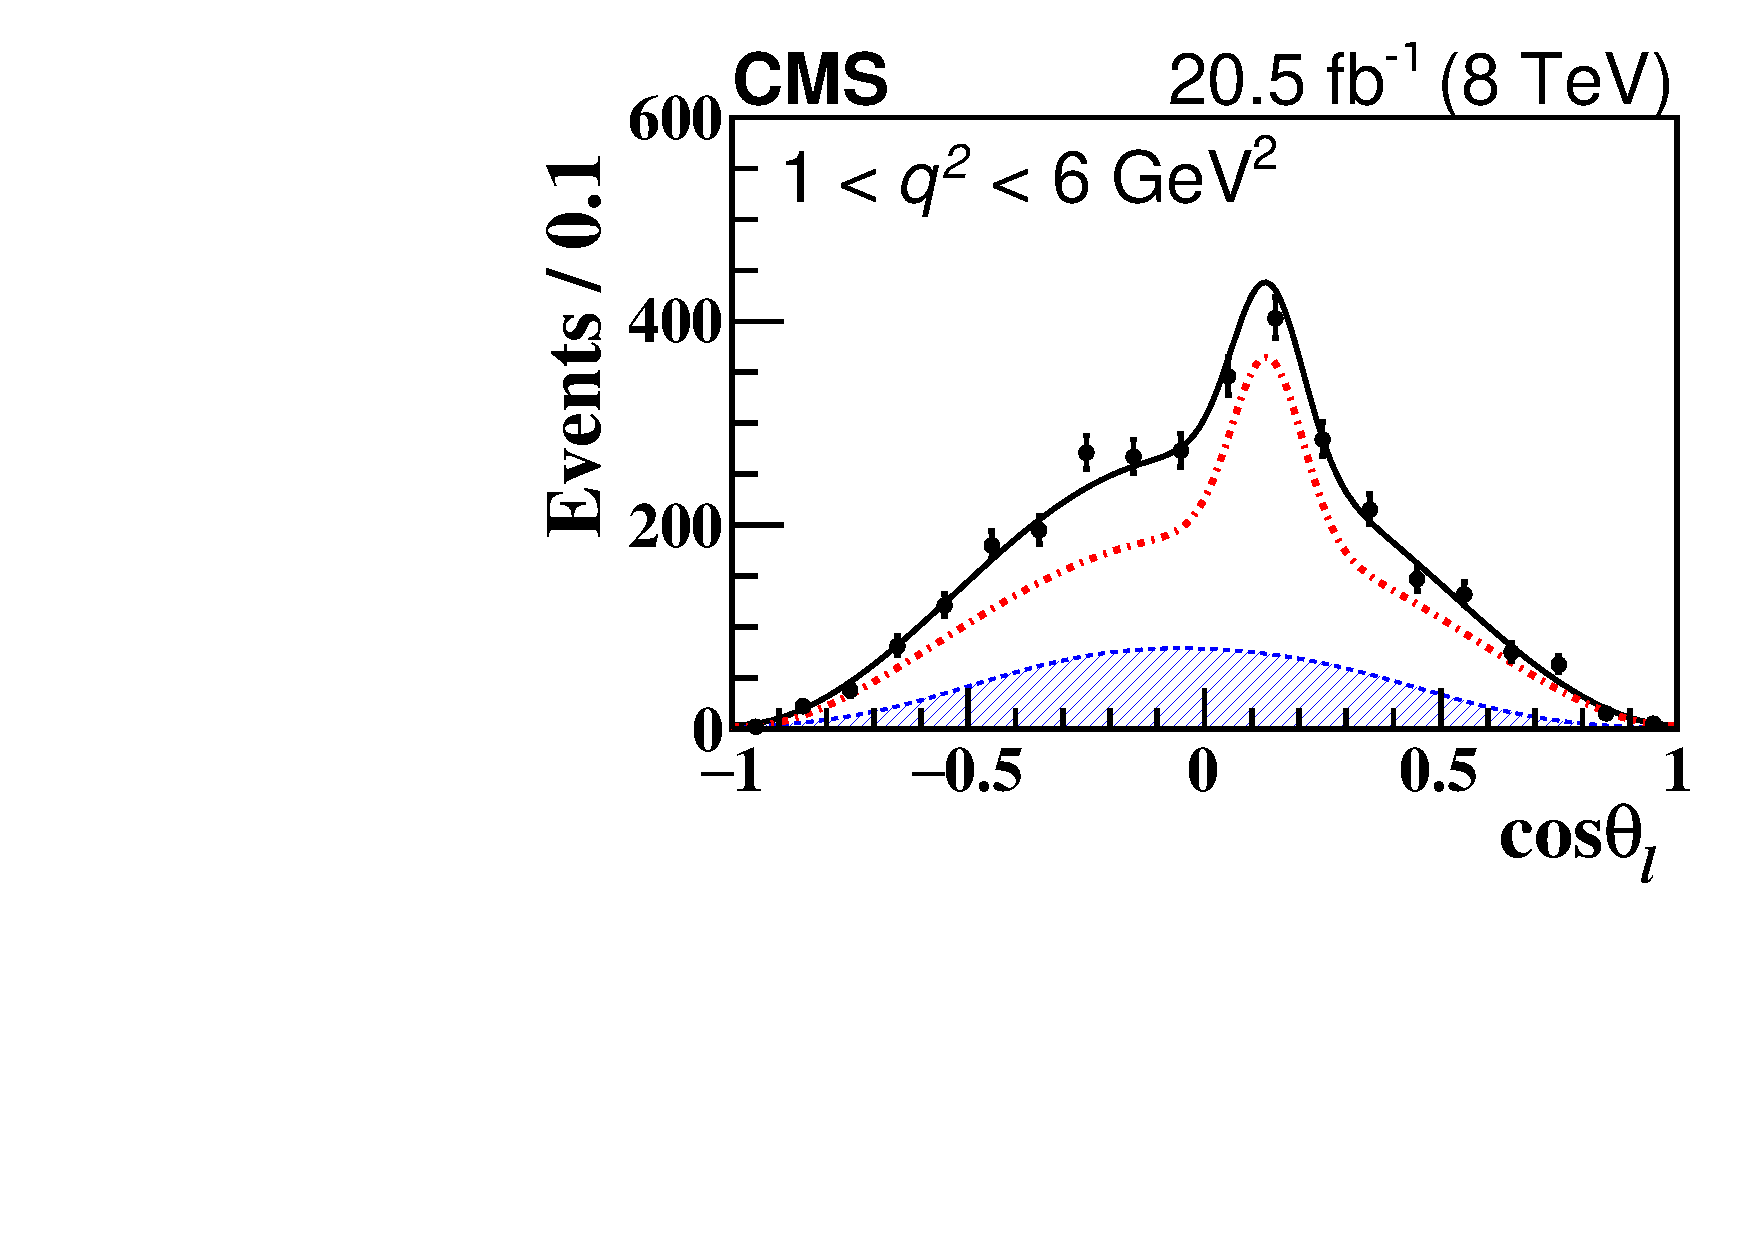
\includegraphics[width=0.45\textwidth]{figures/CMS-BPH-15-001_Figure_004-h}
\caption{
  Projections of the ${\rm K^+\mu^+\mu^-}$ invariant mass distribution (left)
  and the $\cos\theta_\ell$ distribution (right) from the two-dimensional fit
  of data, in the ${\rm 1 < q^2 < 6~GeV^2}$ range~\cite{bph-15-001}. The solid
  lines show the total fit, the shaded area the signal contribution, and the
  dash-dotted lines the background.
}
\label{fig:BPH-15-001_Figures_003-004}
\end{figure}


\begin{figure}[htb]
\centering
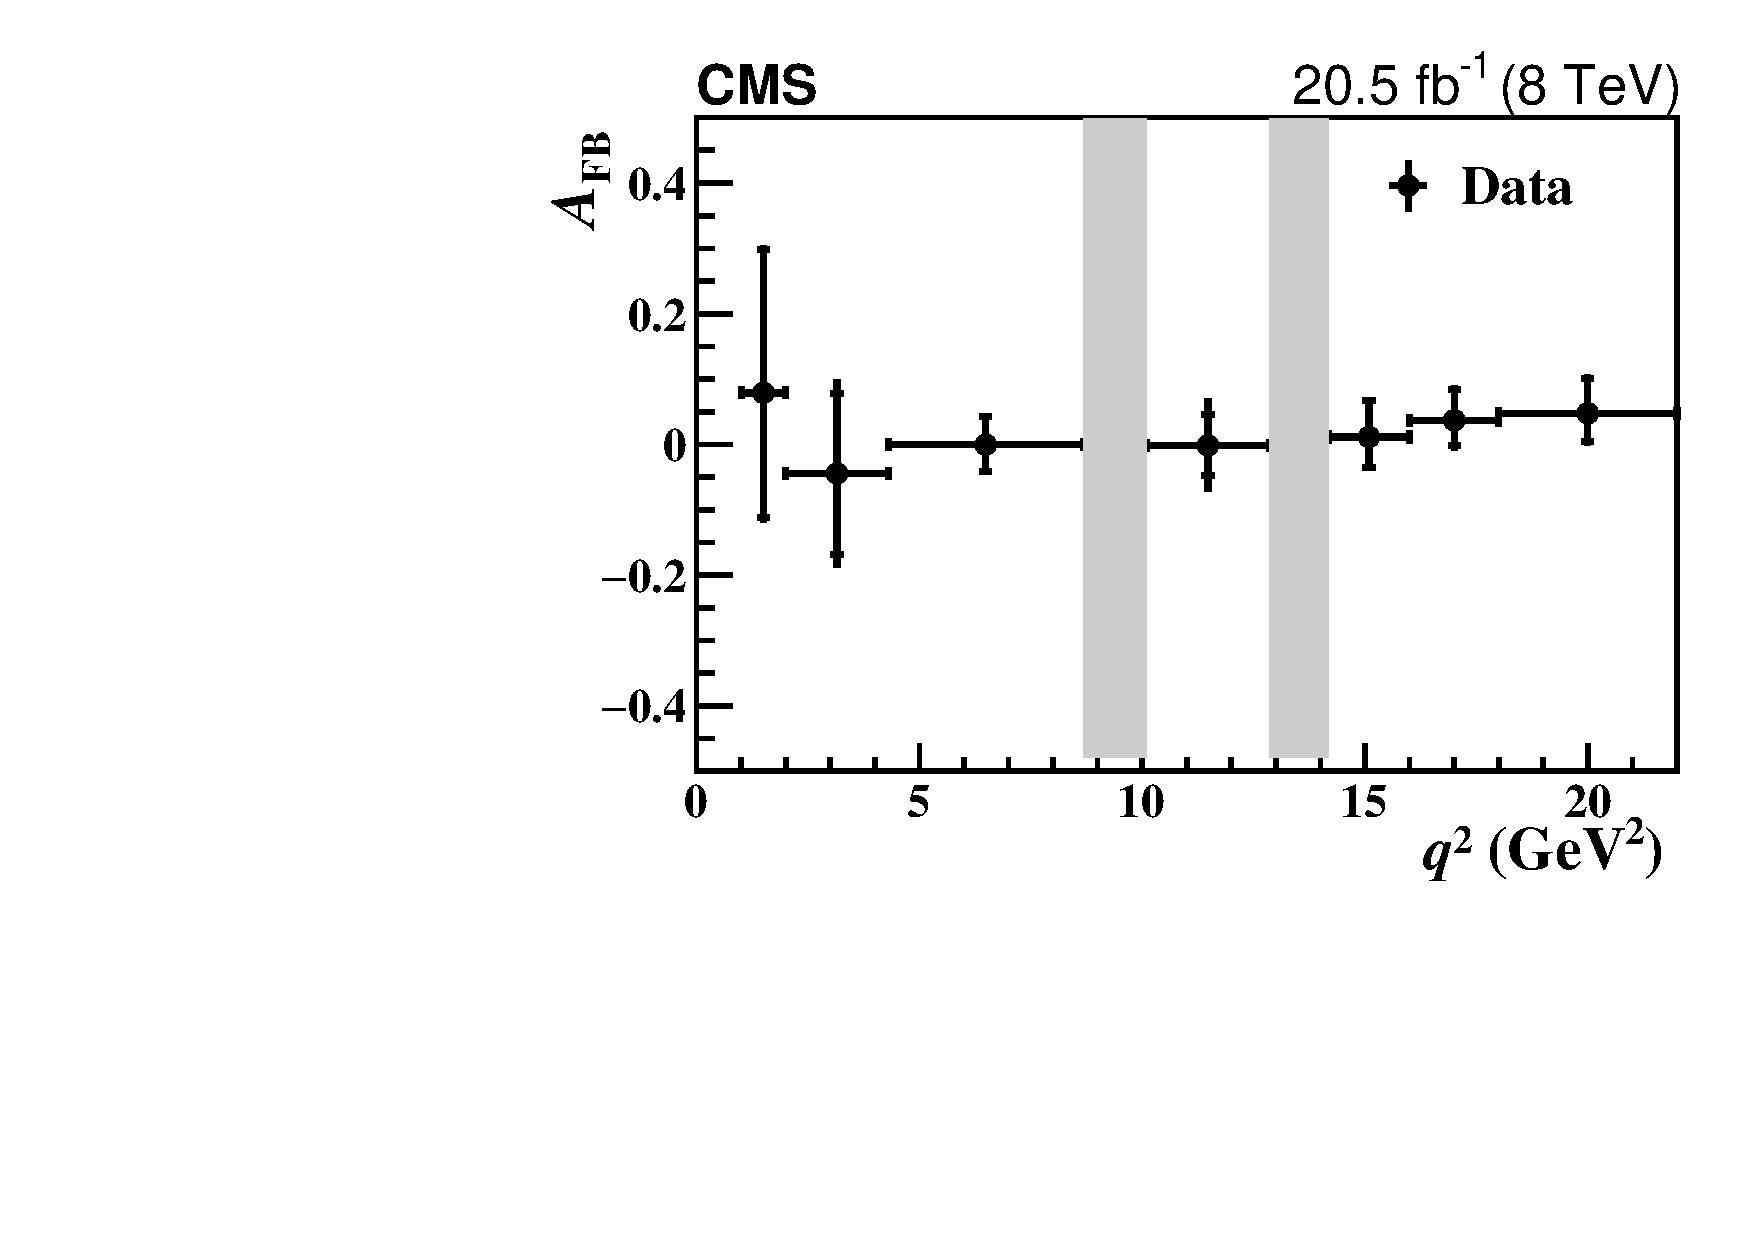
\includegraphics[width=0.45\textwidth]{figures/CMS-BPH-15-001_Figure_005-a}
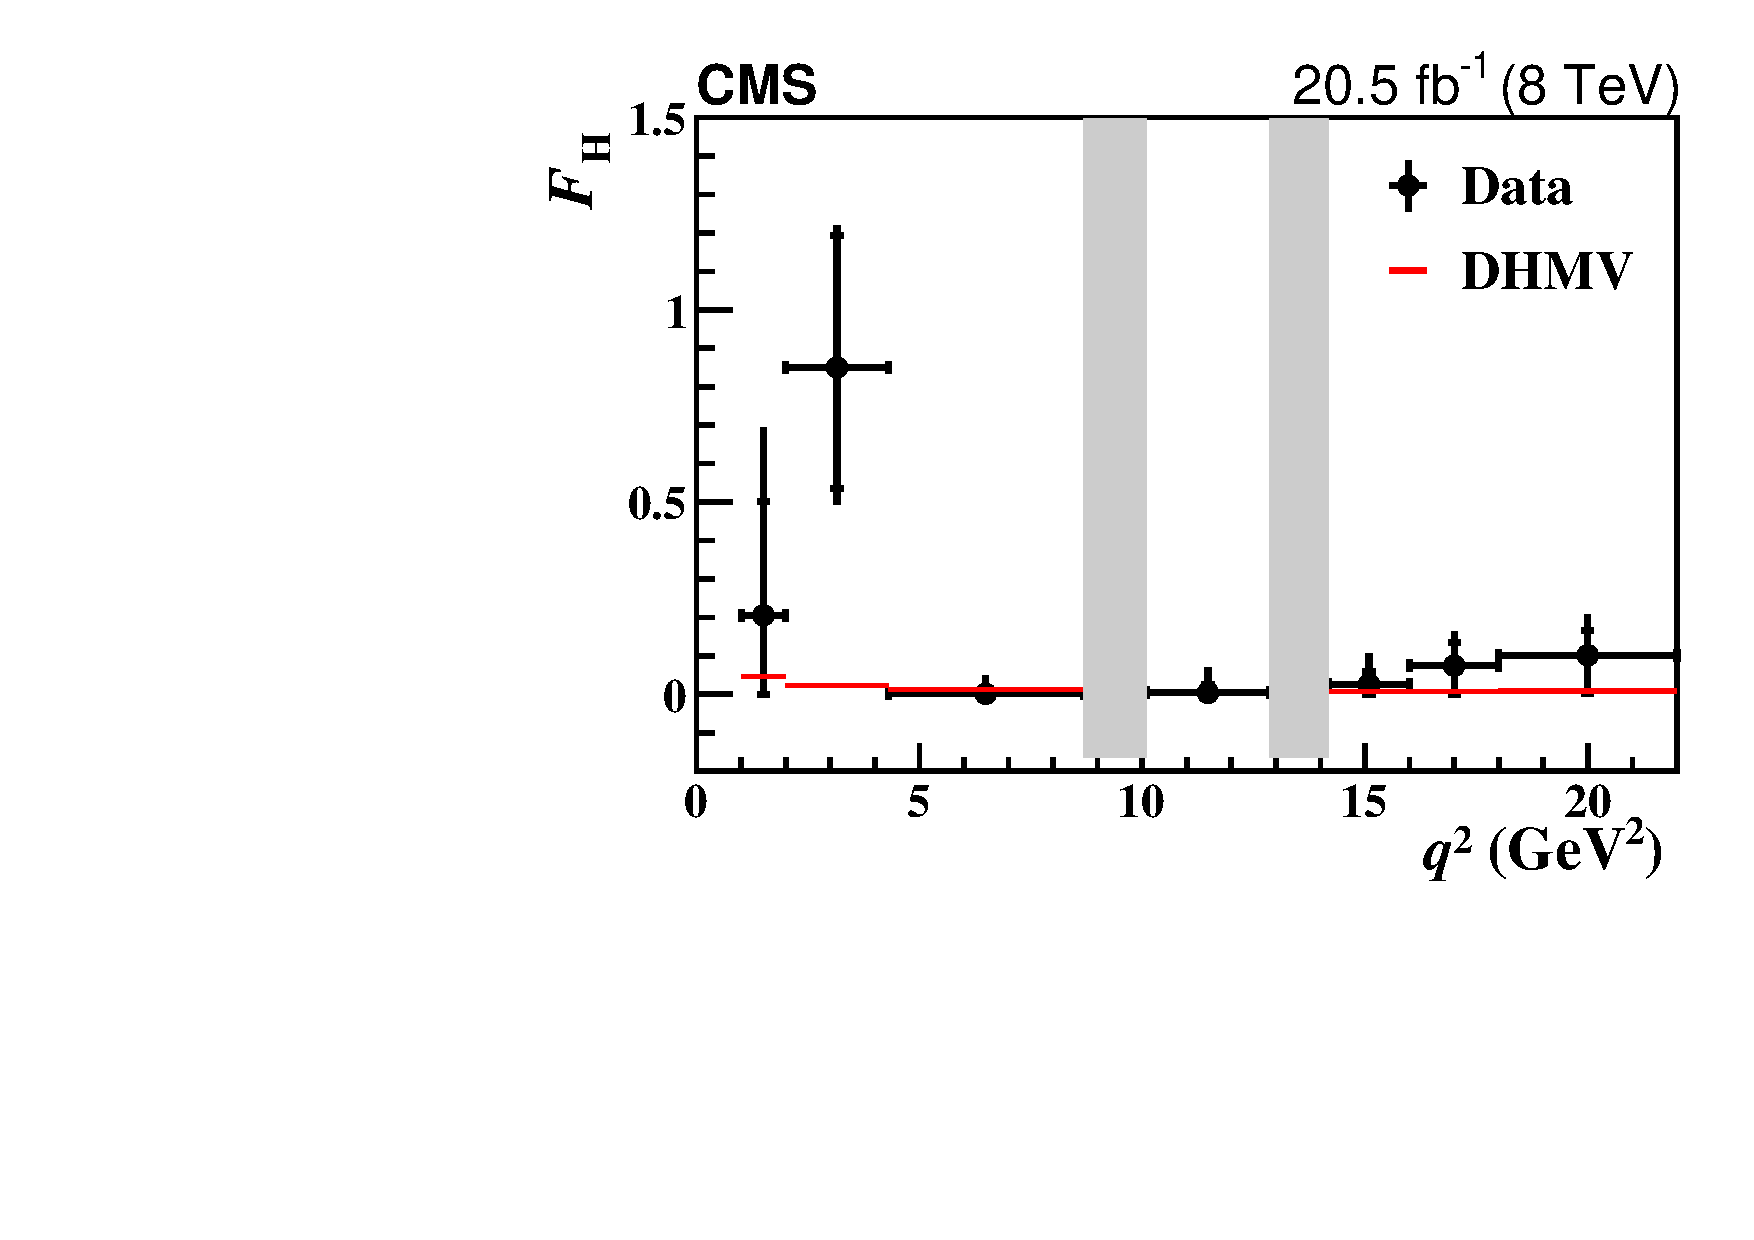
\includegraphics[width=0.45\textwidth]{figures/CMS-BPH-15-001_Figure_005-b}\\
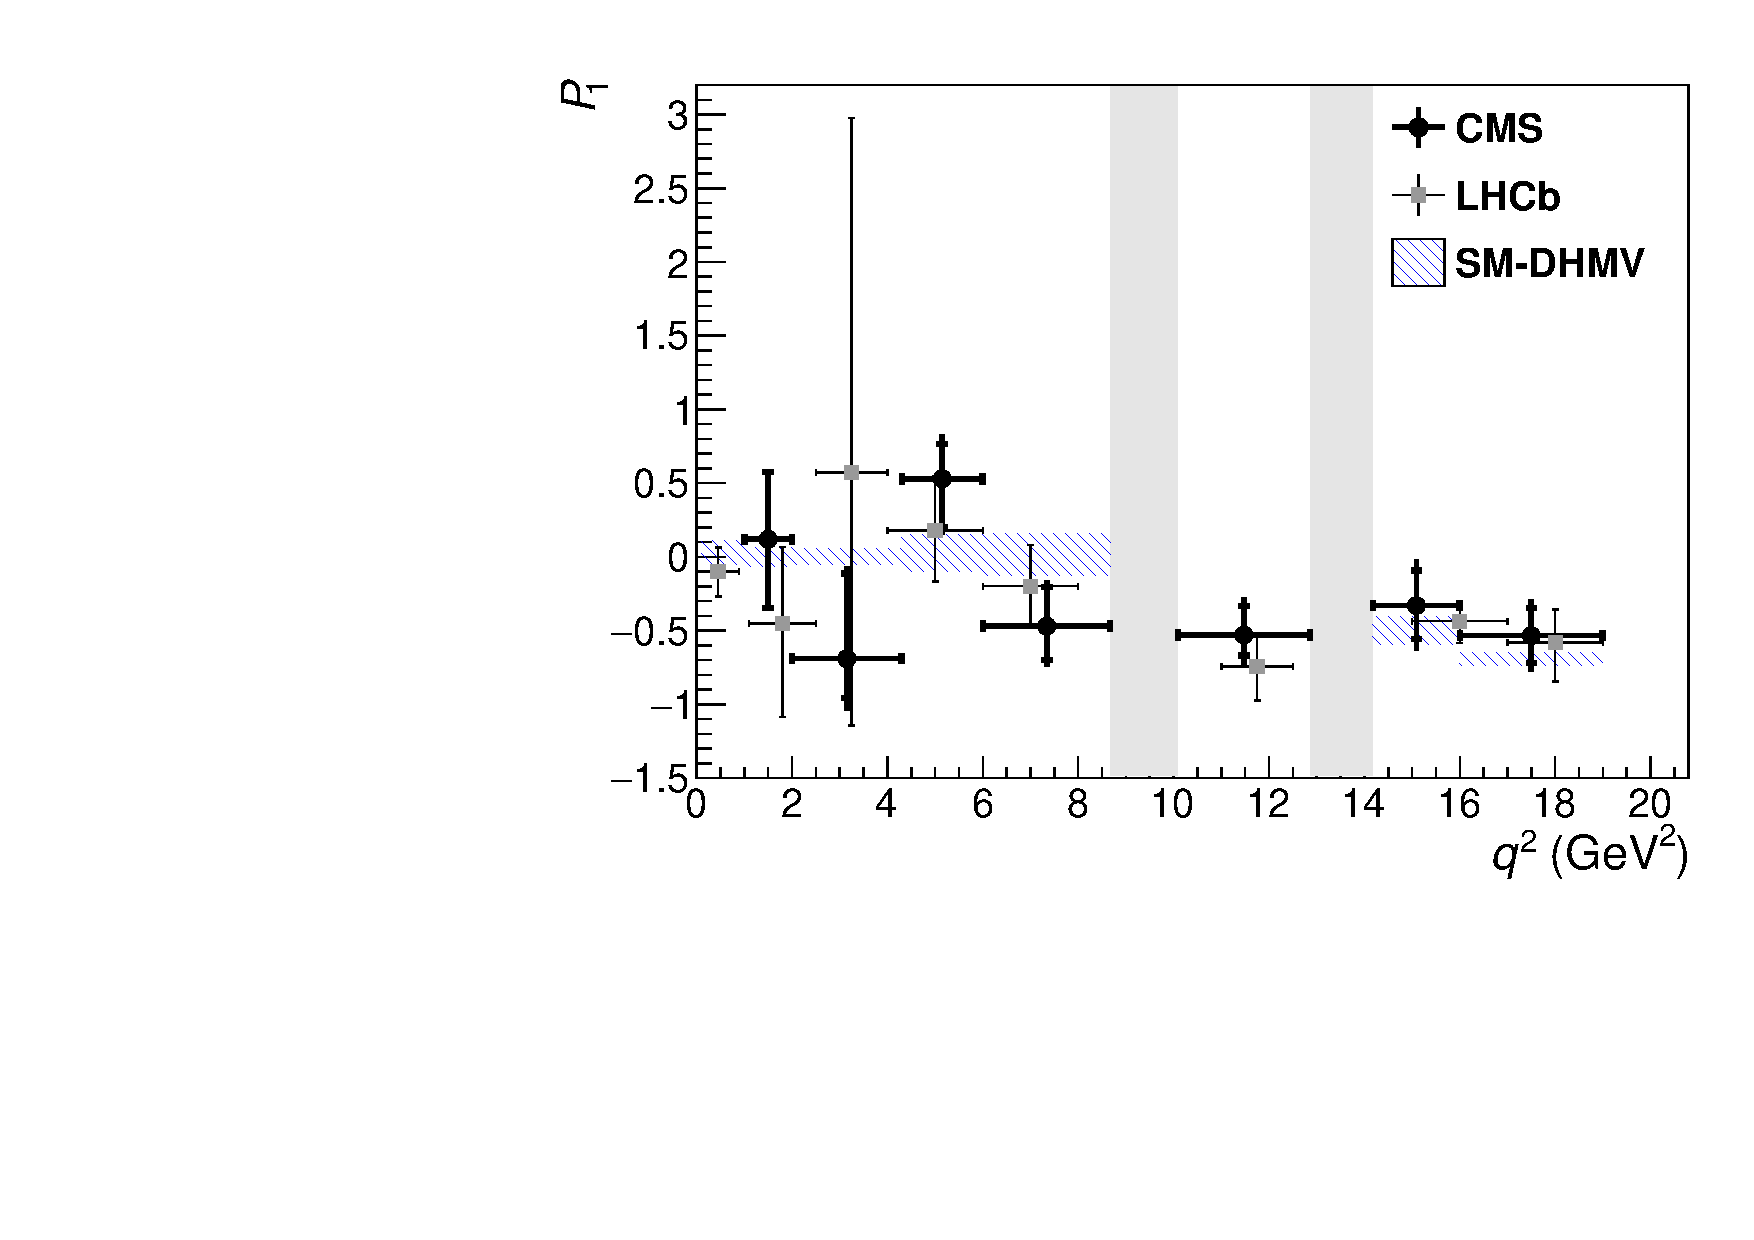
\includegraphics[width=0.45\textwidth]{figures/CMS-BPH-15-008_Figure_003-a}
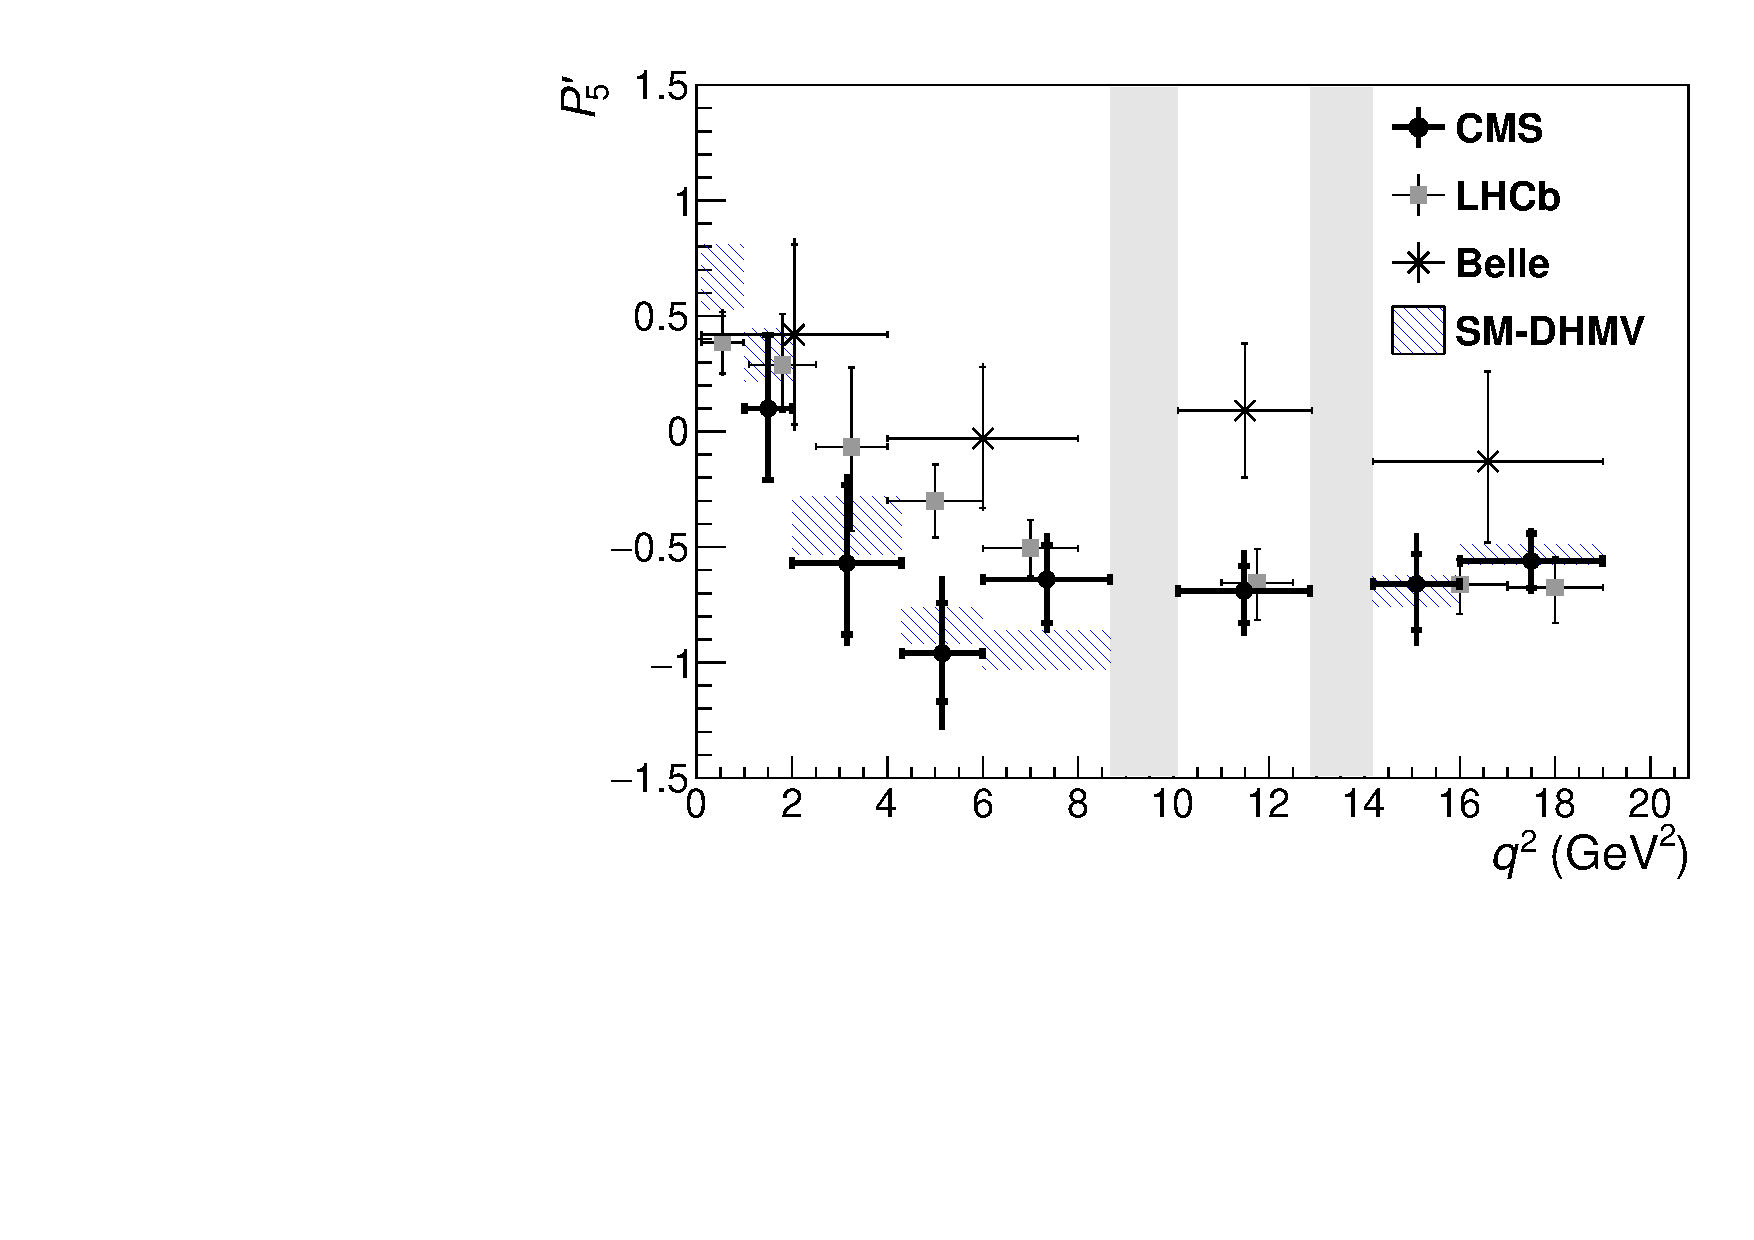
\includegraphics[width=0.45\textwidth]{figures/CMS-BPH-15-008_Figure_003-b}
\caption{
  Measurements of the $A_{\rm FB}$ (top left) and $F_{\rm H}$ (top right)
  parameters versus $q^2$ for ${\rm B^+ \to K^+\mu^+\mu^-}$ decays~\cite{bph-15-001}.
  Measurements of the $P_1$ (bottom left) and $P'_5$ (bottom right) angular
  parameters versus $q^2$ for ${\rm B^0 \to K^{*0}\mu^+\mu^-}$ decays~\cite{bph-15-008}.
  The CMS results are compared to SM  DHMV theoretical
  predictions~\cite{Descotes-Genon:2014uoa,Descotes-Genon:2015uva} and, for the
  $P_1$ and $P'_5$ parameters, they are also compared to results
  from the LHCb~\cite{LHCb} and Belle~\cite{Belle} Collaborations.
}
\label{fig:BPH-15-001_Figure_005__BPH-15-008_Figure003}
\end{figure}


%-------------------------------------------------------------------------------
\section{Angular observables in ${\rm B^0 \to K^{*0}\mu^+\mu^-}$}
%-------------------------------------------------------------------------------

In Reference~\cite{bph-15-008} we study angular distributions of the decay
${\rm B^0 \to K^{*0}\mu^+\mu^-}$ using a sample of proton-proton at the
center-of-mass energy of 8~TeV collected with the CMS detector at the LHC,
corresponding to an integrated luminosity of ${\rm 20.5~fb^{-1}}$. An
angular analysis is performed to determine the $P_1$ and $P'_5$ parameters,
where the $P'_5$ parameter is of particular interest because of recent
measurements that indicate a potential discrepancy with the standard model
predictions~\cite{LHCb,Belle}. Based on a sample of 1397 signal events, the
$P_1$ and $P'_5$ parameters are determined as a function of the dimuon invariant
mass squared, as can be seen in
Figure~\ref{fig:BPH-15-001_Figure_005__BPH-15-008_Figure003}
(bottom distributions). The measurements are in agreement with predictions
based on the standard model.


%-------------------------------------------------------------------------------
\clearpage
\begin{thebibliography}{99}
%-------------------------------------------------------------------------------

\bibitem{top-17-017}
  CMS Collaboration,
  \emph{Search for flavour changing neutral currents in top quark production and decays with three-lepton final state using the data collected at $\sqrt{s} = 13~{\rm TeV}$},
  https://cds.cern.ch/record/2292045, CMS-PAS-TOP-17-017.
\bibitem{cms-detector}
  CMS Collaboration,
  \emph{The CMS experiment at the CERN LHC},
  JINST {\bf 3} S08004 (2008).
\bibitem{top-17-003}
  CMS Collaboration,
  \emph{Search for the flavor-changing neutral current interaction of the top quark and the Higgs boson which decays into a pair of b quarks at $\sqrt{s} = 13~{\rm TeV}$},
  \emph{accepted for publication in JHEP}
  https://cds.cern.ch/record/2296416, CERN-EP-2017-309
  [{\tt arXiv:1712.02399v2}].
\bibitem{cms-atlas-fcnc}
  ATLAS and CMS Collaborations,
  https://twiki.cern.ch/twiki/pub/LHCPhysics/LHCTopWGSummaryPlots/fcnc\_summarybsm\_may18.pdf.
\bibitem{bph-15-001}
  CMS Collaboration,
  \emph{Angular analysis of the decay ${\rm B^+ \to K^+\mu^+\mu^-}$ at ${\rm \sqrt{s} = 8~TeV}$},
  https://cds.cern.ch/record/2621370 CERN-EP-2018-125
  [{\tt arXiv:1806.00636v2}].
\bibitem{bph-15-008}
  CMS Collaboration,
  \emph{Measurement of angular parameters from the decay ${\rm B^0 \to K^{*0}\mu^+\mu^-}$ at ${\rm \sqrt{s} = 8~TeV}$},
  https://cds.cern.ch/record/2287571, CERN-EP-2017-240
  [{\tt arXiv:1710.02846v2}].  
\bibitem{Descotes-Genon:2014uoa}
  S.~Descotes-Genon, L.~Hofer, J.~Matias, and J.~Virto,
  \emph{On the impact of power corrections in the prediction of $B \to K^*\mu^+\mu^-$ observables},
  JHEP {\bf 12} (2014) 125, [{\tt arXiv:1407.8526}].
\bibitem{Descotes-Genon:2015uva}
  S.~Descotes-Genon, L.~Hofer, J.~Matias, and J.~Virto,
  \emph{Global analysis of $b \to s\ell\ell$ anomalies},
  JHEP {\bf 06} (2016) 092, [{\tt arXiv:1510.04239}].
\bibitem{LHCb}
  LHCb Collaboration,
  \emph{Angular analysis of the $B^0 \to K^*\mu^+\mu^- decay using 3~fb^{-1}$ of integrated luminosity},
  JHEP {\bf 02} (2016) 104, [{\tt arXiv:1512:04442}].
\bibitem{Belle}
  Belle Collaboration,
  \emph{Lepton-flavor-dependent angular analysis of $B \to K^* \ell^+\ell^-$},
  Phys. Rev. Lett. {\bf 118} (2017) 111801, [{\tt arXiv:1612.05014}].
\end{thebibliography}

\end{document}
(https://pos.sissa.it/cgi-bin/reader/contribution.cgi?id=PoS(MC2000)002).
